\documentclass[11pt,class=report,crop=false]{standalone}
\usepackage[screen]{../python}



\begin{document}

%====================================================================
\chapitre{Chatgpt -- partie 2}
%====================================================================

% \insertvideo{}{}



\objectifs{Nous poursuivons notre étude de la génération automatique de texte en nous concentrant sur les innovations principales de GPT et en particulier sur le concept d'attention.}



%%%%%%%%%%%%%%%%%%%%%%%%%%%%%%%%%%%%%%%%%%%%%%%%%%%%%%%%%%%%%%%%%%%%%
\section{Architecture}

%--------------------------------------------------------------------
\subsection{Architecture globale et couches du réseau}


\begin{center}
	\begin{minipage}{0.49\textwidth}
		\small	
		\myfigure{0.7}{
			\tikzinput{gpt-01}
		}
	\end{minipage}
	\begin{minipage}{0.49\textwidth}
		
		\myfigure{0.6}{\footnotesize
			\tikzinput{gpt-02}
		}
	\end{minipage}
\end{center}

%--------------------------------------------------------------------
\subsection{Nouveaux concepts}

Les notions de tokenisation et de plongement ont été étudiées au chapitre précédent. Dans cette seconde partie nous nous concentrons sur la notion de transformeur qui est le c\oe ur de réseau et est constituée d'une alternance de couches d'attention et de couches denses. Ces couches sont liées entre elle via le flux résiduel. En sortie du réseau, on obtient un vecteur $w\in \Rr^n$ qu'il faut interpréter comme la liste des mots les plus probables pour compléter la phrase via une opération de retranscription (c'est en quelque sorte l'opération inverse du plongement).

\begin{itemize}
	\item \textbf{Transformeur}. (\emph{Transformer.}) C'est la succession de deux types de couches qui regroupe le principal travail du réseau.
	En entrée on a les vecteurs tokens de $\Rr^n$, $v_1$, $v_2$, \ldots, $v_K$ de la phrase initiale que l'on regroupe comme les colonnes d'une matrice $x_1 \in M_{n,K}$. Chaque couche d'attention et chaque couche dense transforme 
	une matrice $x_i$ en une matrice $x_{i+1}$ de même taille, autrement dit les vecteurs tokens sont modifiés à chaque couche
	
	\item \textbf{Couche d'attention.} Une couche d'attention est composée de plusieurs têtes d'attention. Chaque tête d'attention attribue pour un mot de la phrase un coefficient aux autres mots importants pour comprendre le sens de ce mot. Au lieu de se concentrer seulement sur les derniers mots pour la prédiction du mot suivant, ce mécanisme permet de porter son attention à des mots situés bien avant dans le texte (et d'oublier les mots moins importants).
	
	\item \textbf{Couches denses.} (\emph{MLP}, \emph{Multi-Layer Perceptron.}) Chacune de ces couches est en fait composée de plusieurs sous-couches denses de neurones. On renvoie aux chapitres précédents pour la présentation de ces couches denses que l'on ne réexpliquera pas ici. La dernière sous-couche a $n$ neurones et renvoie donc un vecteur de $\Rr^n$ pour chacun des tokens, c'est-à-dire une matrice de $M_{n,K}$ pour la liste de nos tokens.
	
	\item \textbf{Flux résiduel.} (\emph{Residual stream.})
	Le flux résiduel est une sorte de zone mémoire qui est actualisée après le passage de chaque couche. Il s'agit en fait d'une (très grande) matrice $x_i \in M_{n,K}$ dont les colonnes correspondent aux vecteurs tokens. Chaque couche transforme cette matrice $x_i$ en une matrice $x_{i+1}$. On verra que le choix d'une grande valeur $n$ pour la  dimension permet de stocker dans les vecteurs la position du token dans la phrase et permet aussi d'envoyer de l'information d'une couche à une autre.
	
\end{itemize}

%--------------------------------------------------------------------
\subsection{\emph{GPT2-Small}}

Nous étudierons la variante la plus simple du modèle \emph{GPT2} appelée \emph{GPT2-Small} car son réseau n'a \og{}que\fg{} $117$ millions de poids.
Ce modèle et ses poids sont accessibles publiquement et permet de tester complètement le fonctionnement du réseau sur un ordinateur personnel. 



%%%%%%%%%%%%%%%%%%%%%%%%%%%%%%%%%%%%%%%%%%%%%%%%%%%%%%%%%%%%%%%%%%%%%
\section{Retranscription}


%--------------------------------------------------------------------
\subsection{Retranscription et plongement}

La \defi{retranscription} est l'opération inverse du plongement. Il s'agit d'obtenir un mot, plus précisément un token, à partir d'un vecteur de $\Rr^n$.
Le vocable \emph{retranscription} est la traduction officieuse du terme \emph{unembedding}.

Rappelons que le \defi{plongement} (\emph{embedding}) est une application linéaire 
$\varphi : \Rr^N \to \Rr^n$ définie par $y = \varphi(x) = Ax$
où :
\begin{itemize}
	\item $N$ est le nombre total de tokens ($N=50\,257$ pour \emph{GPT2}),
	\item $n$ est la dimension de plongement ($n=768$ pour \emph{GPT2}),
	\item $A \in M_{n,N}$ est la matrice de plongement, ayant $n$ lignes et $N$ colonnes.
\end{itemize}
Enfin, on rappelle que la base canonique de $\Rr^N$ joue un rôle particulier puisque le $i$-ème vecteur $e_i \in \Rr^N$ de la base canonique correspond au $i$-ème token. Ainsi $v_i = \varphi(e_i) \in \Rr^n$, qui est aussi la $i$-ème colonne de $A$, est le vecteur token associé au token numéro $i$. On renvoie à la première partie pour plus de détail.

La retranscription correspond donc à une fonction $\psi : \Rr^n \to \Rr^N$ qui serait une sorte de réciproque de $\varphi$. À un vecteur $y \in \Rr^n$ (qui n'a pas de signification compréhensible pour un humain), on calcule $x = \psi(y)$ qui correspond à un token, ou plus précisément à une liste de probabilités de chaque token.

Le vecteur $x = (x_1, \ldots, x_N) \in \Rr^N$ s'appelle le vecteur \defi{logit}, ses coordonnées $x_i$ sont des nombres réels qu'il reste difficile à interpréter.
La direction de $x$ correspond au token à obtenir (la norme de $x$ correspond généralement à la confiance que l'on a dans notre résultat). On pourrait chercher quel vecteur identifiant $e_i$ est le plus proche de $x$ (selon la similarité cosinus) afin d'identifier le token numéro $i$ à retranscrire.

On va procéder différemment. On applique à $x$ la fonction softmax, pour obtenir
$$\sigma_i  = \frac{e^{x_i}}{ e^{x_1} + e^{x_2} + \cdots + e^{x_N}} \in [0,1]$$
qui fournit donc une liste $\sigma(x) = (\sigma_1,\ldots,\sigma_N) \in [0,1]^N$.
On interprète ces valeurs $\sigma_i$ comme des probabilités.
On se souvient que chaque coordonnée de $\Rr^N$ correspond exactement à un token.
Ainsi $\sigma_i$ est la probabilité que le vecteur $x$ corresponde au vecteur $e_i$, c'est-à-dire que le token à retranscrire soit le token de numéro $i$.

\myfigure{0.8}{
	\tikzinput{retranscription-02}
} 

\begin{exemple}
Voici un exemple graphique, imaginons que l'on ait transcrit la phrase \og{}\mot{gros félin}\fg{} en un vecteur $y$ de l'espace de tokens $\Rr^n$. Ce vecteur $y$ n'est pas exactement un des vecteurs tokens $v_i$, même s'il est proche du vecteur token $v_i$ correspondant à \mot{lion} et de $v_j$ correspondant à \mot{chat}.

\myfigure{0.6}{
	\tikzinput{retranscription-01}
}

Les coordonnées de $y$ n'ont pas de signification tangible, ni celles de $x = \Psi(y)$ obtenu par retranscription. Ce n'est qu'une fois appliquée la fonction softmax, que l'on peut interpréter le $i$-ème coefficient $p_i$ de $\sigma(x)$ comme la probabilité que le mot codé par $y$ soit le token numéro $i$. Ici le concept \og{}gros félin\fg{} est la combinaison du token \mot{lion} (à 50\%) et du token \mot{chat} (à 40\%), les autres tokens étant peu significatifs.

\myfigure{0.75}{
	\tikzinput{retranscription-03}
}
	
\end{exemple}



\begin{exemple}
\[
x = 
\begin{pmatrix}
2.2 \\ -1.1 \\ 3.3 \\ 0.44	
\end{pmatrix}
\qquad
\sigma(x) = 
\begin{pmatrix}
0.237 \\ 0.008 \\ 0.713 \\ 0.040 
\end{pmatrix}
\]
Ainsi le vecteur $x$ correspond essentiellement au token numéro 3 (à $71\%$) et au token numéro 1 (à $24\%$).	
\end{exemple}

\begin{exemple}
Demandons à \emph{GPT2} de compléter la phrase suivante :
\mycenterline{\mot{The cat sat on the \ldots}}

Voici le vecteur logit $x$ renvoyé pour compléter la phrase, ainsi que sa transformation $\sigma(x)$ par la fonction softmax:
\[
x = \begin{pmatrix}
-94.1504 \\ -91.7648 \\ \vdots \\ -95.7328 \\ -93.9105	

\end{pmatrix} \in \Rr^{50\,257}
\qquad \qquad 
\sigma(x) = \begin{pmatrix}
1.0507 \cdot 10^{-7} \\ 1.1417 \cdot 10^{-6} \\ \vdots \\ 2.1591 \cdot 10^{-8} \\
1.3356 \cdot 10^{-7} 	
\end{pmatrix}\in [0,1]^{50\,257}
\]
La plupart des coefficients $\sigma_i$ de $\sigma(x)$ sont proches de zéro. Il faut identifier les valeurs les plus fortes parmi les $50\,257$ probabilités $\sigma_i$.
Voici le top 5 avec le token correspondant :
\begin{center}
\begin{tabular}{lll}
token id & token & probabilité (en \%) \\ \hline
4314 & \mot{␣floor} & 7.64\%  \\
3996 & \mot{␣bed} & 6.53\%    \\
18507 & \mot{␣couch} & 5.41\%    \\
2323 & \mot{␣ground} & 5.21\%   \\  
5743 & \mot{␣edge} & 4.78\%  \\  	
\end{tabular}
\end{center}


Si on change la phrase à compléter en \mot{The child sat on the \ldots} alors 
les tokens les plus probables sont :
\begin{center}
\begin{tabular}{lll}
token id & token & probabilité (en \%) \\ \hline
3996 & \mot{␣bed} & 13.11\%    \\
4314 & \mot{␣floor} & 11.66\%  \\
18507 & \mot{␣couch} & 7.06\%    \\
34902 & \mot{␣sofa} & 5.06\% \\
2323 & \mot{␣ground} & 4.78\%   \\  	
\end{tabular}
\end{center}
Ainsi \emph{GPT2} sait qu'un enfant va s'asseoir sur son lit alors que le chat s'assoit plutôt par terre !

\end{exemple}



%--------------------------------------------------------------------
\subsection{Retranscription par les moindres carrés}

On exige maintenant en plus que $\psi$ soit une application linéaire.
C'est-à-dire $\psi : \Rr^n \to \Rr^N$, $\psi(y) = By$ où $B \in M_{N,n}$ ($N$ lignes et $n$ colonnes).
Si la matrice $A$ était une matrice inversible (donc en particulier ce serait une matrice carrée avec $N=n$) alors on définirait $\psi$ par $\psi(y) = B y$ où $B = A^{-1}$.
Mais dans notre situation $N$ est très supérieur à $n$, donc la matrice $A$ n'admet pas d'inverse.

Pour un $y \in \Rr^n$ donné, il s'agit donc de trouver $x \in \Rr^N$ tel que $Ax = y$. Mais comme $N$ est très supérieur à $n$, il existe une infinité de tels vecteurs $x$ (les solutions forment un sous-espace affine de dimension $N-n$). Nous allons chercher la solution $x$ qui vérifie $Ax=y$ et telle que sa norme $\| x \|_2$ soit la plus petite possible. 

Nous supposons que la matrice $A$ est de rang $n$ (c'est une hypothèse très raisonnable, qui signifie que les $N$ vecteurs colonnes de $A$ engendrent tout l'espace vectoriel $\Rr^n$). Sous cette hypothèse, la matrice $A A^T \in M_{n,n}$ est inversible, on rappelle que $A^T \in M_{N,n} $ désigne la matrice transposée de $A \in M_{n,N}$ (les lignes et les colonnes sont interverties).
Dans ces conditions nous avons le résultat suivant :
\begin{proposition}
	 Soit $ B = A^T \, (A A^T) ^{-1}$.
	 Soit $y \in \Rr^n$ fixé.
	 Le vecteur $x \in \Rr^N$ tel que $Ax=y$ et $\| x \|_ 2$ soit minimale est donné par $x_{\min} = By$.
\end{proposition}

Il faut bien faire attention que nous ne sommes pas dans le cas le plus fréquent de la méthode des moindres carrés d'un système sur-dimensionné pour lequel on aurait $n \ge N$. Ici le système linéaire $Ax=y$ est sous-dimensionné car $N \ge n$.

Ici il est très facile de vérifier que $x_{\min}$ est solution de $Ax=y$ (montrer que la norme est minimale demande une petite preuve).
Géométriquement, le sous-espace affine $Ax=y$ est parallèle au sous-espace vectoriel $Ax=0$. Le vecteur $x_{\min}$ solution est la projection orthogonale du vecteur nul $0$ sur ce sous-espace affine.

\myfigure{1}{
	\tikzinput{retranscription-04}
}

\begin{exemple}
Soit $n=2$ et $N=4$. Considérons le problème $Ax=y$ avec :
$$A = \begin{pmatrix}
1 & 2 & 0 & -1 \\
1 & 1 & -1 & 0 \\
\end{pmatrix} \in M_{n,N}
\qquad\qquad
y = \begin{pmatrix}
2 \\ -1	
\end{pmatrix} \in \Rr^n$$

Alors on calcule :
$$A^T = \begin{pmatrix}
 1 & 1 \\
 2 & 1 \\
 0 & -1 \\
-1 & 0 \\
\end{pmatrix} \in M_{N,n}
\qquad
A A^T =\begin{pmatrix}
6 & 3 \\
3 & 3 \\
\end{pmatrix} \in M_{n,n}
\qquad
(A A^T)^{-1}  = \frac13 \begin{pmatrix}
	1 & -1 \\
	-1 & 2 \\
\end{pmatrix} \in M_{n,n}
$$
Ainsi :
$$
B  = A^T \, (A A^T) ^{-1} = 
\frac13 
\begin{pmatrix}
0 & 1 \\
1 & 0 \\
1 & -2 \\
-1 & 1 \\	
\end{pmatrix} \in M_{N,n}
$$
Et donc :
$$x_{\text{min}} 
= B y = 
\frac13
\begin{pmatrix}
-1 \\ 2 \\ 4 \\ -3	
\end{pmatrix} \in \Rr^N
$$

\end{exemple}

%--------------------------------------------------------------------
\subsection{Retranscription par apprentissage}

Voyons comment la retranscription s'effectue dans les modèles de langage comme \emph{GPT2}.
Considérons le réseau de neurones suivant.

\myfigure{0.8}{
	\tikzinput{retranscription-05}
}

En entrée nous avons un vecteur $x \in \Rr^N$. Après une couche dense de $n$ neurones (sans biais, sans activation) nous obtenons un vecteur $y \in \Rr^n$ qui correspond à une transformation linéaire $y  = Ax$ (où les coefficients de $A \in M_{n,N}$ correspondent aux poids de cette couche). Notons $\varphi : x \mapsto y$ ce plongement, dans notre contexte le vecteur $y$ est le vecteur token.
On enchaîne avec une seconde couche dense de $N$ neurones. On obtient un vecteur $z \in \Rr^N$ défini par $z = B y$ où $B \in M_{N,n}$ est une matrice (les coefficients de $B$ sont les poids de cette seconde couche). Notons $\psi : y \mapsto z$.
On entraîne maintenant ce réseau sur les bi-grammes comme dans le chapitre précédent. Les poids des deux couches définissent respectivement les coefficients des matrices $A$ et $B$. 
Par notre entraînement, la fonction
$F : \Rr^N \to \Rr^N$ associe à un token $x$, le token suivant $y$, ou plus précisément le logit que l'on transforme en une liste de probabilités pour le token suivant.
Ainsi le plongement $\varphi$ et la retranscription $\psi$ sont déterminés par apprentissage.
Vu la construction qui vise à prédire le token suivant, il n'y a aucune raison que plongement et retranscription soient des opérations inverses l'une de l'autre. C'est le cas dans toutes les architectures modernes de réseau de neurones : plongement et retranscription ne sont pas symétriques.

Les deux couches que l'on vient de construire sont le début et la fin d'un réseau pour les grands modèles de langage. Entre ces deux couches on va intercaler des couches d'attention et d'autres couches de neurones.



%%%%%%%%%%%%%%%%%%%%%%%%%%%%%%%%%%%%%%%%%%%%%%%%%%%%%%%%%%%%%%%%%%%%%
\section{Flux résiduel}

%--------------------------------------------------------------------
\subsection{Motivation}

\mycenterline{\emph{\og{}La mémoire c'est l'attention au fil du temps.\fg{}}}

Cette phrase d'Alex Graves, spécialiste des réseaux de neurones,
résume bien l'idée nouvelle qui fait fonctionner les grands modèles de langage.

Revenons en arrière et prenons un réseau de neurones composé d'une succession de couches (denses ou de convolution). L'information ou l'abstraction qu'aurait apprise une couche au début se dilue au fil des couches suivantes. On renvoie au chapitre 
\og{}Convolution avec tensorflow/keras\fg{} et sa section \og{}Que voit un réseau de neurones ?\fg{}.

De plus, si on enchaîne un grand nombre de couches on risque de buter sur le problème des gradients trop petits (\emph{vanishing gradient problem}). La rétropropagation modifie, via le gradient, d'abord les poids des dernières couches, puis en remontant vers les premières couches le gradient a tendance à devenir de plus en plus petit, il se rapproche de zéro ce qui fait que les poids des premières couches n’évoluent presque plus.

Le \emph{flux résiduel} est une façon de conserver le savoir acquis au fil des couches et de pouvoir le transmettre directement à n’importe laquelle des couches suivantes, même si elle se situe beaucoup plus loin dans le réseau.

Ainsi, chaque bloc va pouvoir se spécialiser (certains s’occupent d’interpréter les positions entre les tokens, d’autres des verbes, d’autres de la syntaxe\ldots).
Le flux résiduel rassemble ce travail d’équipe et surtout, comme énoncé dans la citation, retient ce qui est important et oublie le reste.



%--------------------------------------------------------------------
\subsection{Principe}

Voici le schéma de principe général du flux résiduel. Chaque token $t$ de la phrase d'entrée correspond à un vecteur $v$.
La phrase de $K$ tokens est transformée en $K$ vecteurs de $\Rr^n$.
Dans toute la suite on va identifier $K$ vecteurs $v_1,v_2,\ldots,v_K$ de $\Rr^n$ à une matrice $x \in M_{n,K}$ (avec $n$ lignes et $K$ colonnes) dans laquelle chaque colonne est l'un des vecteurs $v_j$.


\myfigure{1}{
	\tikzinput{flux-01}
} 

Le bloc numéro $i$ reçoit du flux résiduel en entrée une liste de $K$ vecteurs de $\Rr^n$ $(v_1,v_2, \ldots,v_K)$ qui est donc une matrice $x_i \in M_{n,K}$.
Le bloc transforme cette matrice $x_i$ en une autre matrice $y_i \in M_{n,K}$. Cette matrice $y_i$ est ajoutée au flux résiduel, c'est-à-dire $x_{i+1} = x_i + y_i$.
Autrement dit, chaque bloc transforme les vecteurs de plongement $v_j$. 

\myfigure{0.7}{
	\tikzinput{flux-02}
} 


C'est une façon un peu étrange de conserver dans $x_{i+1}$ la trace de $x_i$. On aurait plutôt tendance à imaginer un système plus explicite, par exemple conserver la paire $(x_i,y_i)$, mais cette méthode devient vite trop lourde puisqu'on ajouterait des données à chaque étape. On va profiter ici que l'espace $\Rr^n$ est de grande dimension (par exemple $n=768$) afin que l'information contenue dans $x_i$ ne soit pas écrasée dans $x_{i+1}$. Comme d'habitude avec les réseaux de neurones, on laisse l'apprentissage faire le tri de ce qui est important ou pas.

Il y a deux types de blocs : les blocs d'attention et les blocs de couches denses de neurones. Ces blocs alternent, par exemple dans \emph{GPT2} il y a $12$ blocs de chaque type.
\begin{itemize}
	\item Chaque bloc d'attention est en fait composé de $12$ sous-blocs d'attention (\emph{attention head}) qui modifient les vecteurs tokens en fonction de leur position dans la phrase. Nous y reviendrons en détail.
	
	\item Les blocs de neurones (\emph{MLP} pour \emph{Multi-Layer Perceptron}) sont des couches de neurones denses classiques. Pour \emph{GPT2} chacun de ces blocs est composé des deux couches de neurones : une première couche de $3072$ neurones (qui recoivent $n=768$ entrées via chaque vecteur colonne $v \in \Rr^n$ de $x_i$) et une seconde de $768$ neurones qui renvoie donc un vecteur de taille $n=768$ et correspond à une colonne de $y_i$.
	
\end{itemize}


Voyons maintenant comment chaque bloc interagit avec le flux résiduel.
Notons $x \mapsto b_i(x)$ l'action du bloc d'attention ou du bloc de couches denses.
Nous ajoutons une transformation linéaire en entrée et en sortie de chaque bloc.

Soit $W_{\text{in}}^i \in M_{n,n}$ une matrice de taille $n \times n$. Elle transforme un vecteur $v \in \Rr^n$ en un vecteur $w = W_{\text{in}}^i v \in \Rr^n$.
Elle agit aussi sur une matrice $x \in M_{n,K}$ (chaque colonne de $W_{\text{in}}^i x \in M_{n,K}$ est l'image de la colonne correspondante de $x$).
De même, soit $W_{\text{out}}^i \in M_{n,n}$ correspondant à $x \mapsto W_{\text{out}}^i x$ de $M_{n,K}$ dans $M_{n,K}$.

Les coefficients des matrices $W_{\text{in}}^i$ et $W_{\text{out}}^i$ sont des poids du réseau global et sont donc déterminés par apprentissage.

La matrice $x_{i+1}$ (vue comme juxtaposition de vecteurs colonnes) du flux résiduel après l'action du bloc $i$ est définie par la formule de récurrence :
$$x_{i+1} = x_i \  + \ W_{\text{out}}^i \cdot b_i \cdot W_{\text{in}}^i x_i$$

\emph{Note.} L'écriture est un peu abusive car $b_i$ n'est pas une matrice mais une fonction non linéaire, l'écriture correcte serait $x_{i+1} = x_i + W_{\text{out}}^i \cdot b_i \big( W_{\text{in}}^i x_i \big)$.


On comprend facilement que le bloc $i$ envoie presque directement sa sortie vers l'entrée du bloc $i+1$, via la transformation linéaire de matrice 
$ W_{\text{in}}^{i+1} \cdot W_{\text{out}}^i$.

\myfigure{0.7}{
	\tikzinput{flux-03}
} 


%--------------------------------------------------------------------
\subsection{Calculs}

Il est plus intéressant de se rendre compte qu'un bloc $i$ peut assez facilement transmettre des informations à n'importe quel bloc $j$ situé après ($j > i$).
En jouant sur les sous-espaces de $\Rr^n$, on va voir comment on pourrait envoyer un vecteur de la sortie du bloc $i$ vers l'entrée du bloc $j$ via le produit :
$$W_{\text{in}}^{j} \cdot W_{\text{out}}^i.$$

\myfigure{0.7}{
	\tikzinput{flux-04}
}

Expliquons comment faire sur un exemple où le bloc $1$ envoie des données au bloc $3$ sans interférence du bloc $2$.

Considérons par exemple la matrice $W_{\text{out}}^1$, $W_{\text{out}}^2$ et $W_{\text{in}}^3$ définie par blocs :
\[
W_{\text{out}}^1 = 
\left(\begin{array}{@{}c|c@{}}
	X & (0)  \\
	\hline
	(0) & \tilde X	
\end{array}\right)
\qquad
W_{\text{out}}^2 = 
\left(\begin{array}{@{}c|c@{}}
	(0) & (0)  \\
	\hline
	(0) & \tilde Y	
\end{array}\right)
\qquad
W_{\text{in}}^3 = 
\left(\begin{array}{@{}c|c@{}}
	Z & (0)  \\
	\hline
	(0) & \tilde Z	
\end{array}\right)
\]
Dans chaque matrice, le bloc en haut à gauche est une matrice de taille $p \times p$.
La matrice $W_{\text{in}}^2$ elle, est quelconque.
Notons $\Rr^p \subset \Rr^n$ le sous-espace vectoriel correspondant au bloc en haut à gauche. On peut décomposer n'importe quel vecteur $x \in \Rr^n$ sous la forme $x = (u, v)$ où $u \in \Rr^p$ et $v \in \Rr^{n-p}$.
On s'intéresse maintenant uniquement au sous-espace $\Rr^p$ :
\begin{itemize}
	\item Le bloc $1$ va ajouter un vecteur du type $u_2 = X u_1$ sur le sous-espace $\Rr^p$ du flux résiduel.
	\item Le bloc $2$ ne va pas modifier le sous-espace $\Rr^p$ du flux résiduel, du fait de la matrice nulle comme premier bloc de $W_{\text{out}}^2$, ainsi le flux résiduel ne change pas $u_3 = u_2$.
	\item Ainsi le bloc $3$ reçoit le vecteur $u_3 = u_2 = X u_1$, exactement comme si le bloc $2$ n'existait pas.
\end{itemize}

Bien sûr ici nous avons conçu à priori la structure qui permet de passer d'un bloc à un bloc futur. Dans la réalité c'est l'apprentissage qui détermine les coefficients des matrices qui sont des poids du réseau et il est sûrement difficile de comprendre quelles informations passent d'un bloc à l'autre sur un réseau entraîné.


%--------------------------------------------------------------------
\subsection{Sortie finale}


Après la dernière couche, le flux résiduel contient la matrice $x_\ell \in M_{n,K}$.
On obtient ainsi $K$ vecteurs tokens que l'on transforme en un seul par une combinaison linéaire :
$$w_{\text{sortie}} = x_\ell \cdot C  \in \Rr^n \qquad \text{ où } \ C \in M_{K,1}$$
Les coefficients de la matrice $C$ sont des poids du réseau. 
Le vecteur sortie $w_{\text{sortie}} \in \Rr^n$ est ensuite transformé en une liste de tokens probables par la retranscription.


%%%%%%%%%%%%%%%%%%%%%%%%%%%%%%%%%%%%%%%%%%%%%%%%%%%%%%%%%%%%%%%%%%%%%
\section{Plongement de position}

%--------------------------------------------------------------------
\subsection{Motivation}

Les règles de syntaxe et de grammaire ne sont pas expliquées à l'avance dans les grands modèles récents de langages.
On laisse le modèle découvrir ces règles tout seul par apprentissage. C'est évidemment là que la position joue un rôle primordial afin, par exemple, de comprendre la structure sujet/verbe/complément dans la phrase \og{}Le chat mange le fromage.\fg{}.

Le plongement du token numéro $t$ est un vecteur $v(t) \in \Rr^n$.
On a vu au chapitre précédent que de tels vecteurs tokens sont regroupés selon la signification du token.
Mais une phrase c'est bien plus que l'ensemble de ses mots ! Les phrases \og{}Le chat course la souris.\fg{} et \og{}La souris course le chat.\fg{} sont composées des mêmes mots mais leurs sens sont biens distincts.


Nous nous intéressons donc maintenant à la position des mots dans une phrase.
Pour une phrase donnée, on commence par la découper sous la forme d'une liste de mots, ou plus exactement d'une liste ordonnée de tokens $(t_1,t_2,\ldots,t_K)$.
À chacun des ces tokens est associé un vecteur token $v(t_k) \in \Rr^n$. On associe donc à la phrase une matrice $V = ( v(t_1), v(t_2), \ldots, v(t_k) ) \in M_{n,K}$ dont chaque colonne est un vecteur token.

\myfigure{1}{
	\tikzinput{position-01}
} 


La matrice $V$ tient bien compte de la position des tokens dans la phrase, mais lors son passage à travers le réseau de neurones la matrice $V$ va subir de nombreuses transformations et en particulier des colonnes vont être mélangées, il n'y aura donc plus de traces de l'ordre.
On pourrait ajouter à côté de chaque vecteur token sa position dans la phrase : $(v(t_k), k)$ ; mais ce ne serait pas adapté à notre tactique qui consiste à effectuer tous les calculs dans $\Rr^n$.

L'idée que l'on va mettre en œuvre est de coder la position numéro $k$ par un vecteur $w_k \in \Rr^n$.
Quel est alors le plongement global du token $t_k$ se trouvant à la position $k$ dans une phrase ?
C'est tout simplement le vecteur somme :
\mycenterline{$u_k = v(t_k) + w_k$}

On rappelle que $v(t_k) \in \Rr^n$ est le vecteur token, il ne dépend que du mot/token $t_k$ et que $w_k \in \Rr^n$ est un vecteur position qui ne dépend que de la position $k$.

Cela peut sembler une façon étrange de procéder puisque en superposant deux données on risque de perdre de l'information.
Mais d'une part, il faut se souvenir que les vecteurs appartiennent à l'espace $\Rr^n$ de grande dimension donc il y a de la place.
D'autre part le vecteur $v(t_k)$ est déterminé par rétropropagation en tenant compte de ce système de position, donc un bon apprentissage permettra de reconstituer à la fois $v(t_k)$ et la position $k$ à partir de $u_k$.


%--------------------------------------------------------------------
\subsection{Formule}

\begin{itemize}
	\item Soit $n$ la dimension de plongement voulue ($n$ doit être pair, par exemple $n=768$ pour \emph{GPT2}).
	
	\item Soit $p$ un grand entier arbitraire fixé ($p=10\,000$ pour \emph{GPT2}). 
\end{itemize}

Pour $i \ge 0$, on pose :
$$\omega_i = \frac{1}{p^\frac{2i}{n}}.$$
Pour $k \ge 0$, on définit le \defi{vecteur position} :
\[ w_k = 
\begin{pmatrix}
  \cos(	\omega_0 k ) \\
  \sin(	\omega_0 k ) \\
  \cos(	\omega_1 k ) \\
  \sin(	\omega_1 k ) \\
	\vdots \\
  \cos(	\omega_{n/2-1} k ) \\
  \sin(	\omega_{n/2-1} k ) \\	  
\end{pmatrix}
\in \Rr^n
\]

\begin{exemple}
Pour $K=4$, $n=6$ et $p=100$, les vecteurs positions sont :
$$w_0 = 
\begin{pmatrix}
1 \\ 0 \\ 1 \\ 0 \\ 1 \\ 0	
\end{pmatrix}
\qquad
w_1 = 
\begin{pmatrix}
0.540 \\ 0.841 \\ 0.976 \\ 0.213 \\ 0.998 \\ 0.046
\end{pmatrix}
\qquad
w_2 = 
\begin{pmatrix}
-0.416 \\  0.909 \\ 0.908 \\  0.417 \\  0.995 \\  0.0926
\end{pmatrix}
\qquad
w_3 = 
\begin{pmatrix}
-0.989 \\   0.141 \\  0.798 \\  0.602 \\ 0.990 \\ 0.138	
\end{pmatrix}
$$
\end{exemple}


\emph{Remarques.} Dans la pratique on a une phrase de $K$ tokens ou moins ($K=1024$ pour \emph{GPT2}). Il faut décider si on compte les tokens en démarrant de $k=0$ à $K-1$ ou de $k=1$ à $K$ mais on verra que cela n'a pas d'importance. 
Enfin, toujours pour \emph{GPT2}, dans le vecteur $w_k$, les sinus sont placés avant les cosinus, on verra pourquoi notre choix est préférable pour les explications mathématiques.


%--------------------------------------------------------------------
\subsection{Justifications}

\textbf{Justification via l'informatique.}

L'écriture binaire  est une façon de représenter un entier $k\ge0$ sous la forme d'un vecteur (les chiffres binaires étant les coefficients).
Le chiffre des unités se calcule par $b \, \% \,2$, le chiffre suivant par $(b/\!/2) \ \% \, 2$, etc.

Par exemple l'écriture binaire de $k=22$ est $10110$ (le chiffre des unités étant tout à droite) et donnerait le vecteur $w = \left(\begin{smallmatrix}0 \\ 1 \\ 1 \\ 0 \\ 1 \end{smallmatrix}\right)$.

Plus généralement si $b$ désigne la base ($b=2$ pour le binaire, $b=10$ pour l'écriture décimale) alors le $i$-ème chiffre de $k$ en base $b$ est :
\[
c_i = (k /\!/ b^i) \, \% \, b
\]
où on rappelle que $a /\!/ b$ désigne le quotient de la division euclidienne de $a$ par $b$ et $a \, \% \, b$ son reste.

Dans notre formule, on retrouve le terme $k / q^i$ où ici $q = p^{\frac{2}{n}}$. Et la fonction sinus (ou cosinus) joue le rôle de la fonction périodique (comme la réduction modulo $b$ qui est périodique).

\bigskip


\textbf{Justification via la physique.}

Étudions la fonction $(k,i) \mapsto \sin( i \omega_k)$ comme un signal.

On peut tracer les fonctions $k \mapsto \sin( i \omega_k)$ pour différentes valeurs de $i$ fixées. Il s'agit de sinusoïdes, la valeur de la période dépend du paramètre $i$.

\begin{center}
	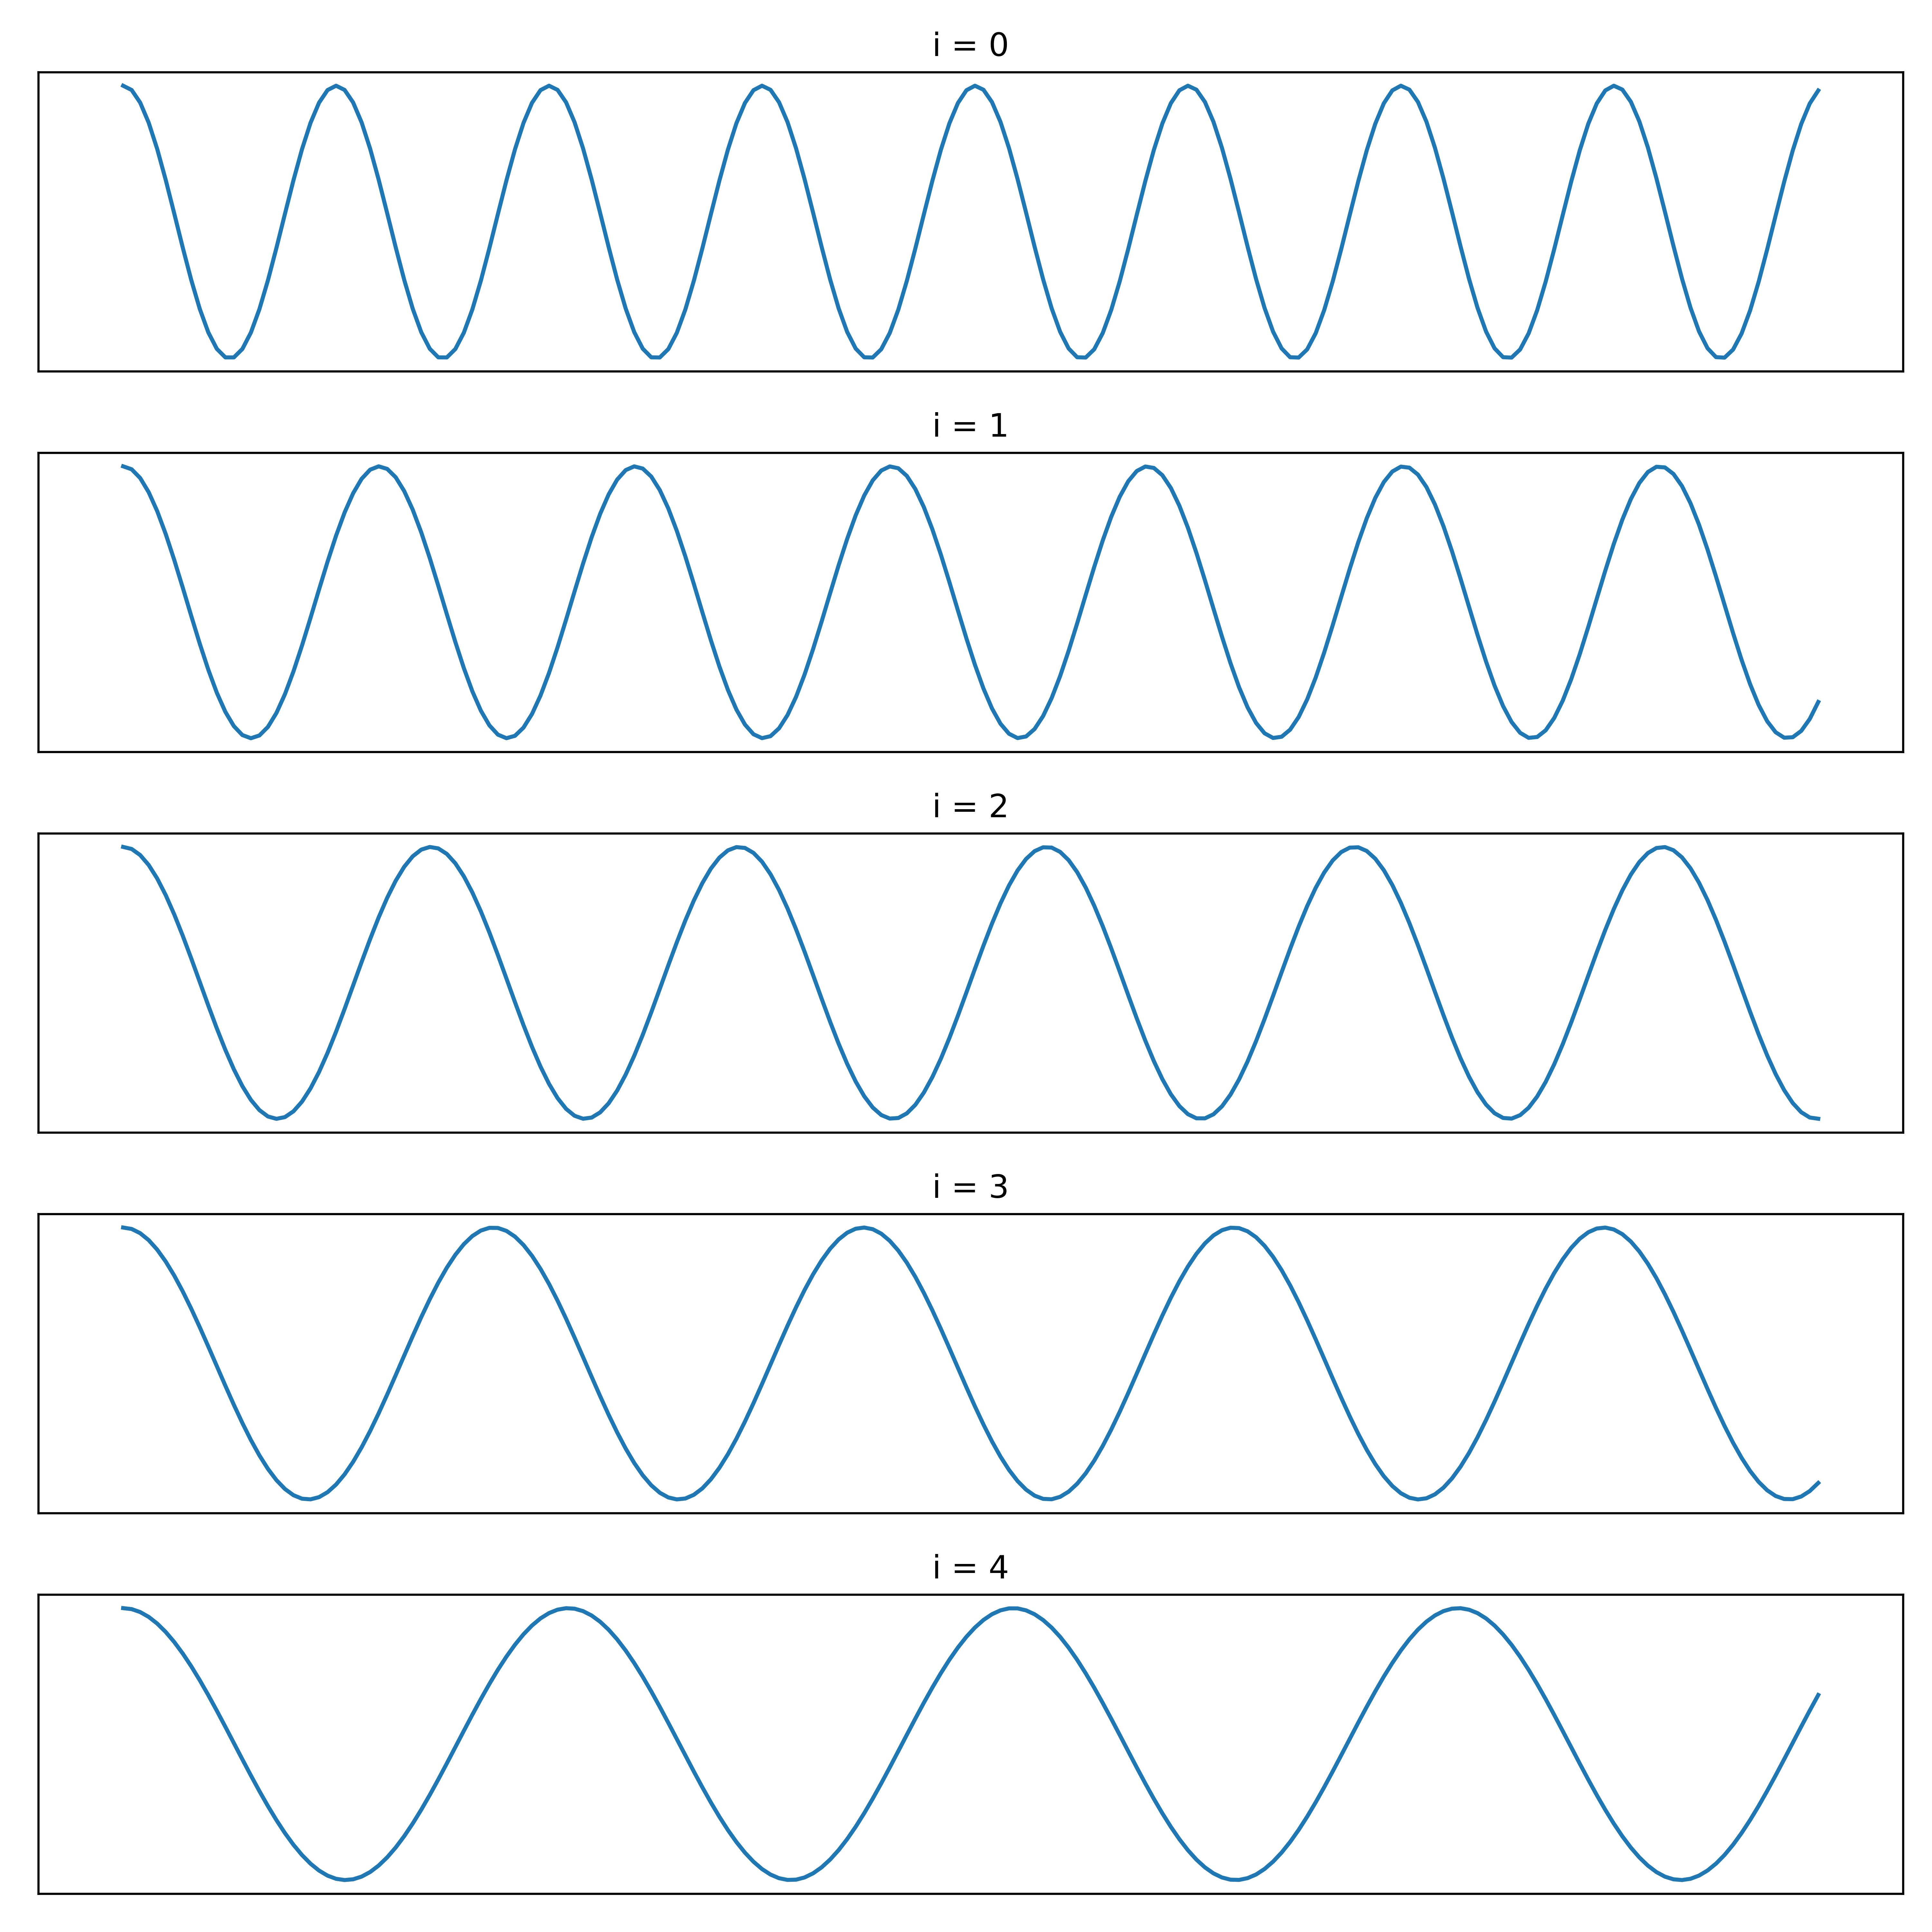
\includegraphics[scale=\myscale,scale=0.4]{figures/position-icst}
\end{center}

Si on trace les fonctions $i \mapsto \sin( i \omega_k)$ pour différentes valeurs de $k$ fixées. Ce sont des fonctions oscillantes entre $-1$ et $+1$ mais les oscillations ralentissent lorsque $i$ croît. Ainsi connaissant un tel graphe on peut retrouver la valeur de $k$. Autrement dit le vecteur $w_k$ détermine  la position $k$ (assez facilement d'un point de vue numérique).

\begin{center}
	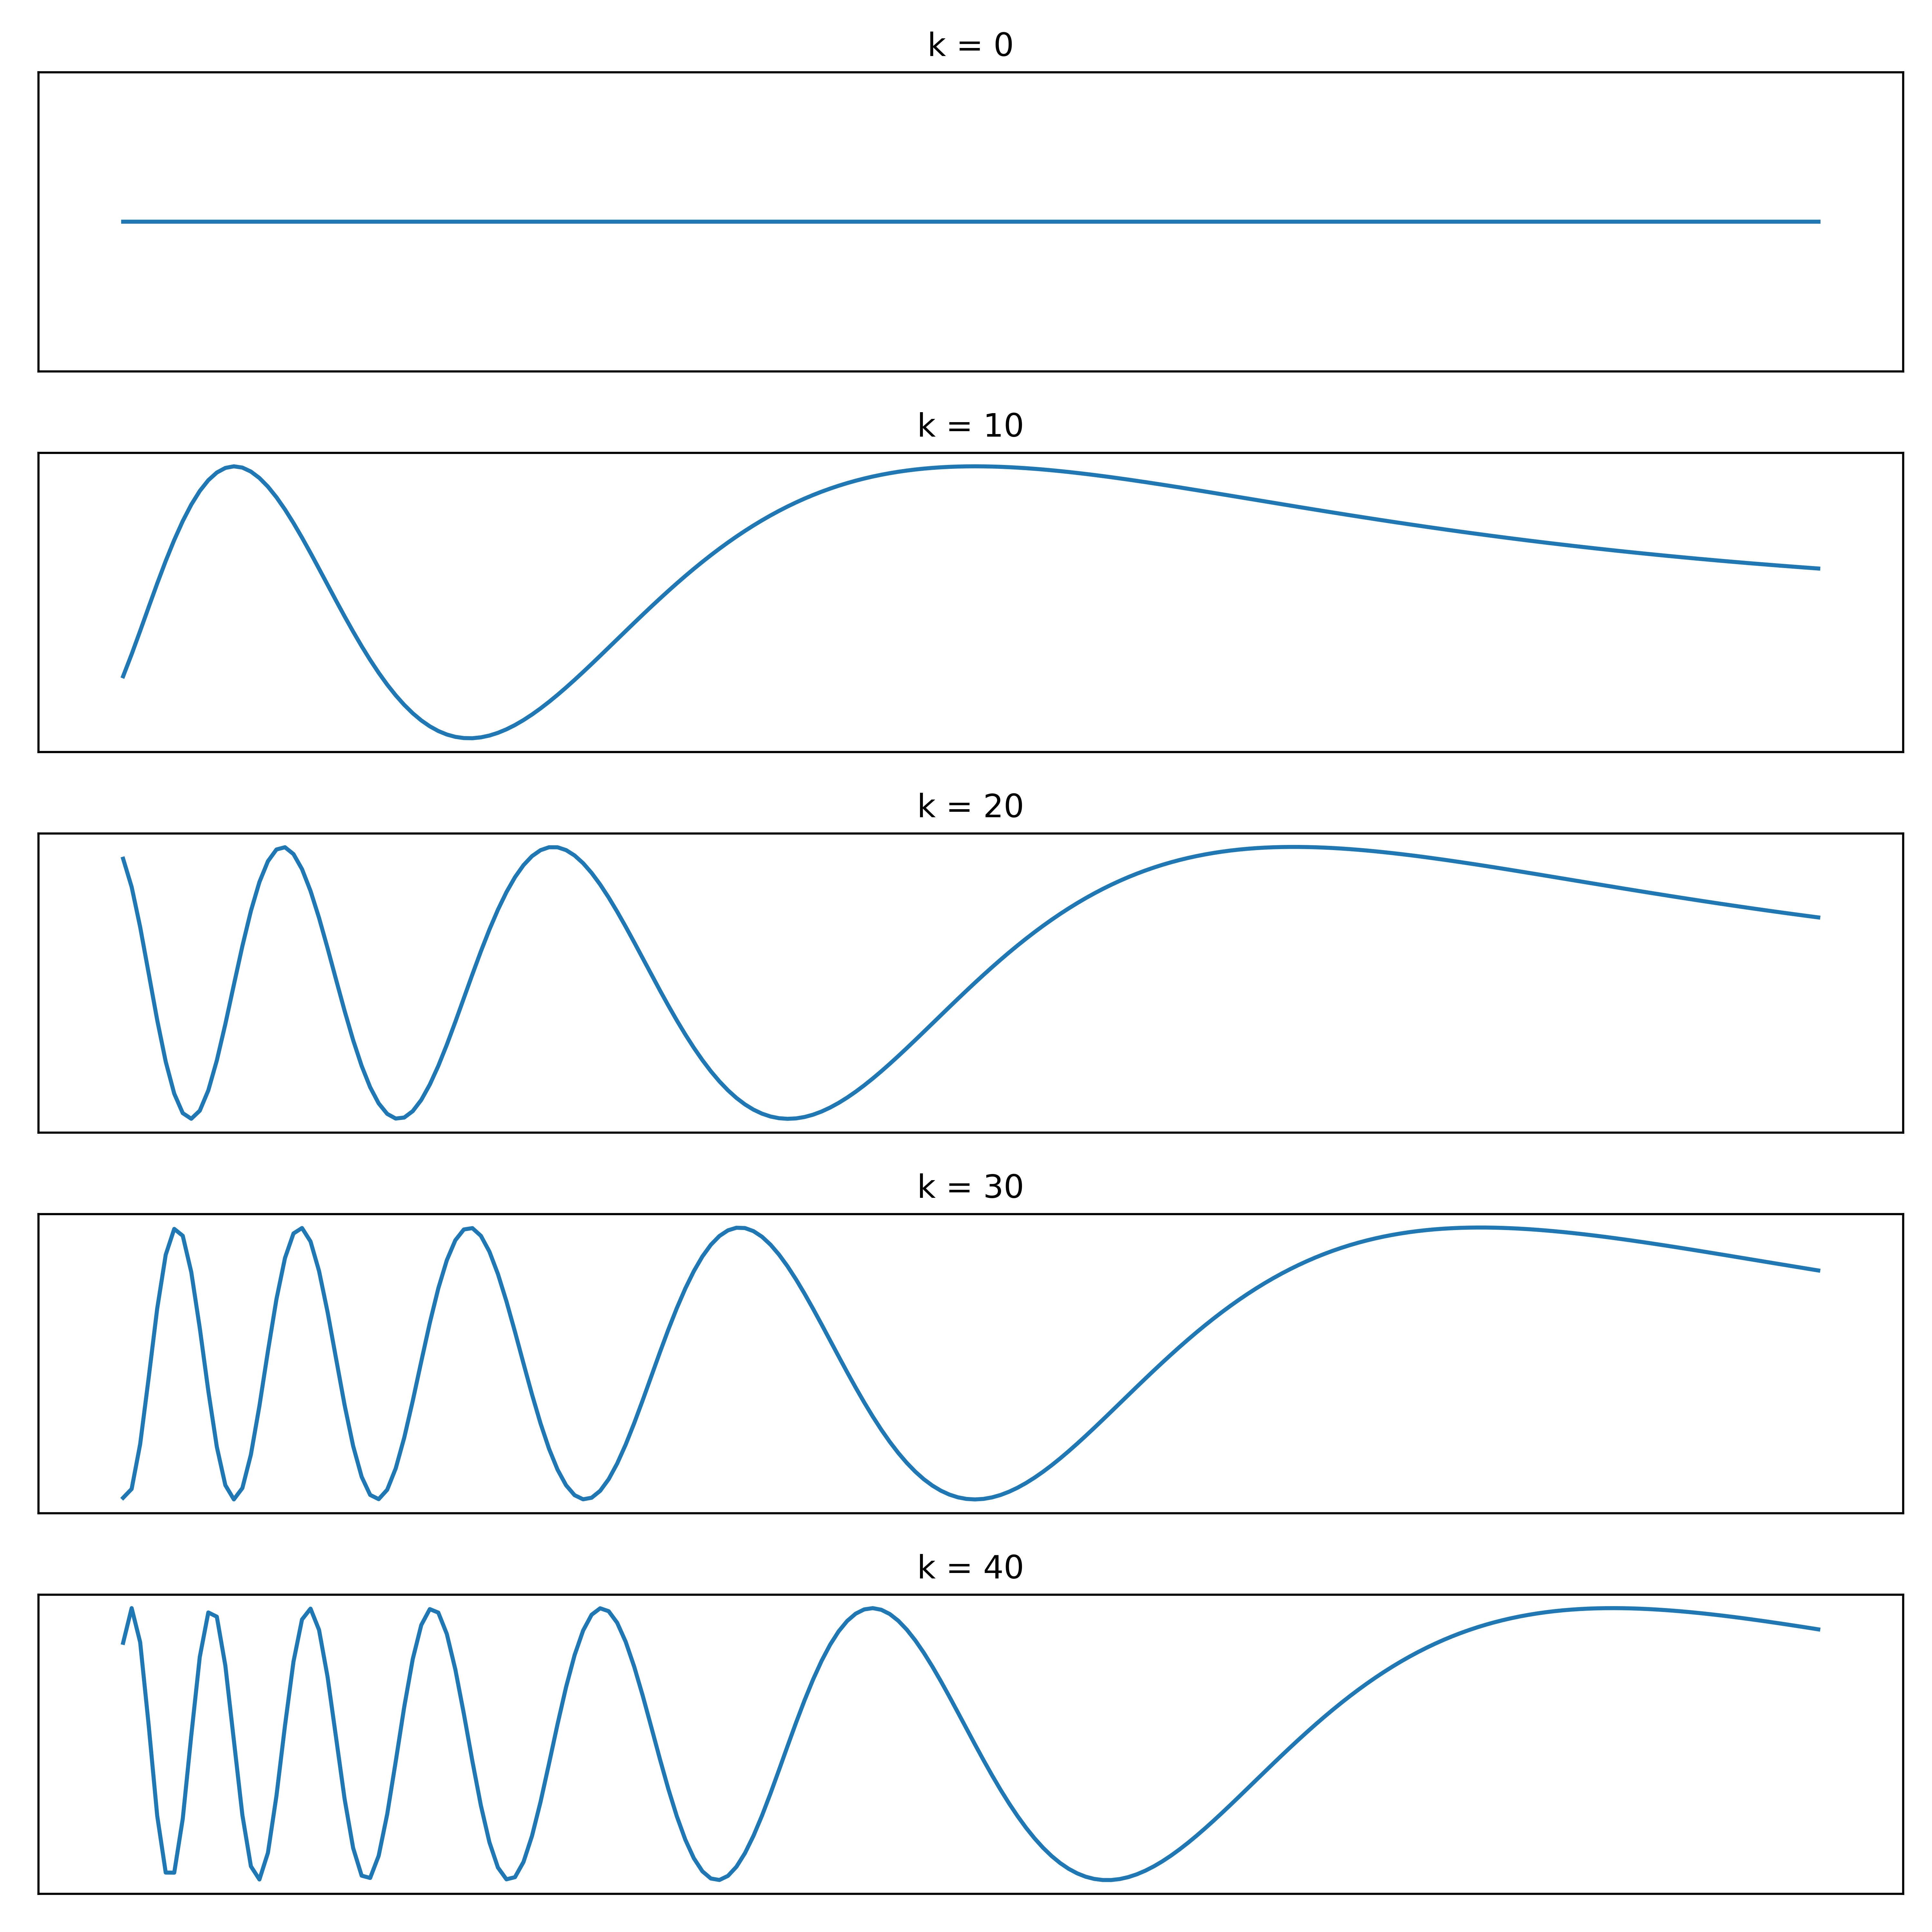
\includegraphics[scale=\myscale,scale=0.4]{figures/position-kcst}
\end{center}

\bigskip

\textbf{Justification via les mathématiques.}

On peut considérer la fonction $(k,i) \mapsto \sin( i \omega_k)$ comme une fonction de deux variables. Ci-dessous, voici la \emph{heatmap} (les couleurs correspondent aux valeurs de la fonction). Chaque colonne correspond à une valeur de $k$, les colonnes sont suffisamment différentes les unes des autres pour pouvoir déterminer la valeur de $k$.

\begin{center}
	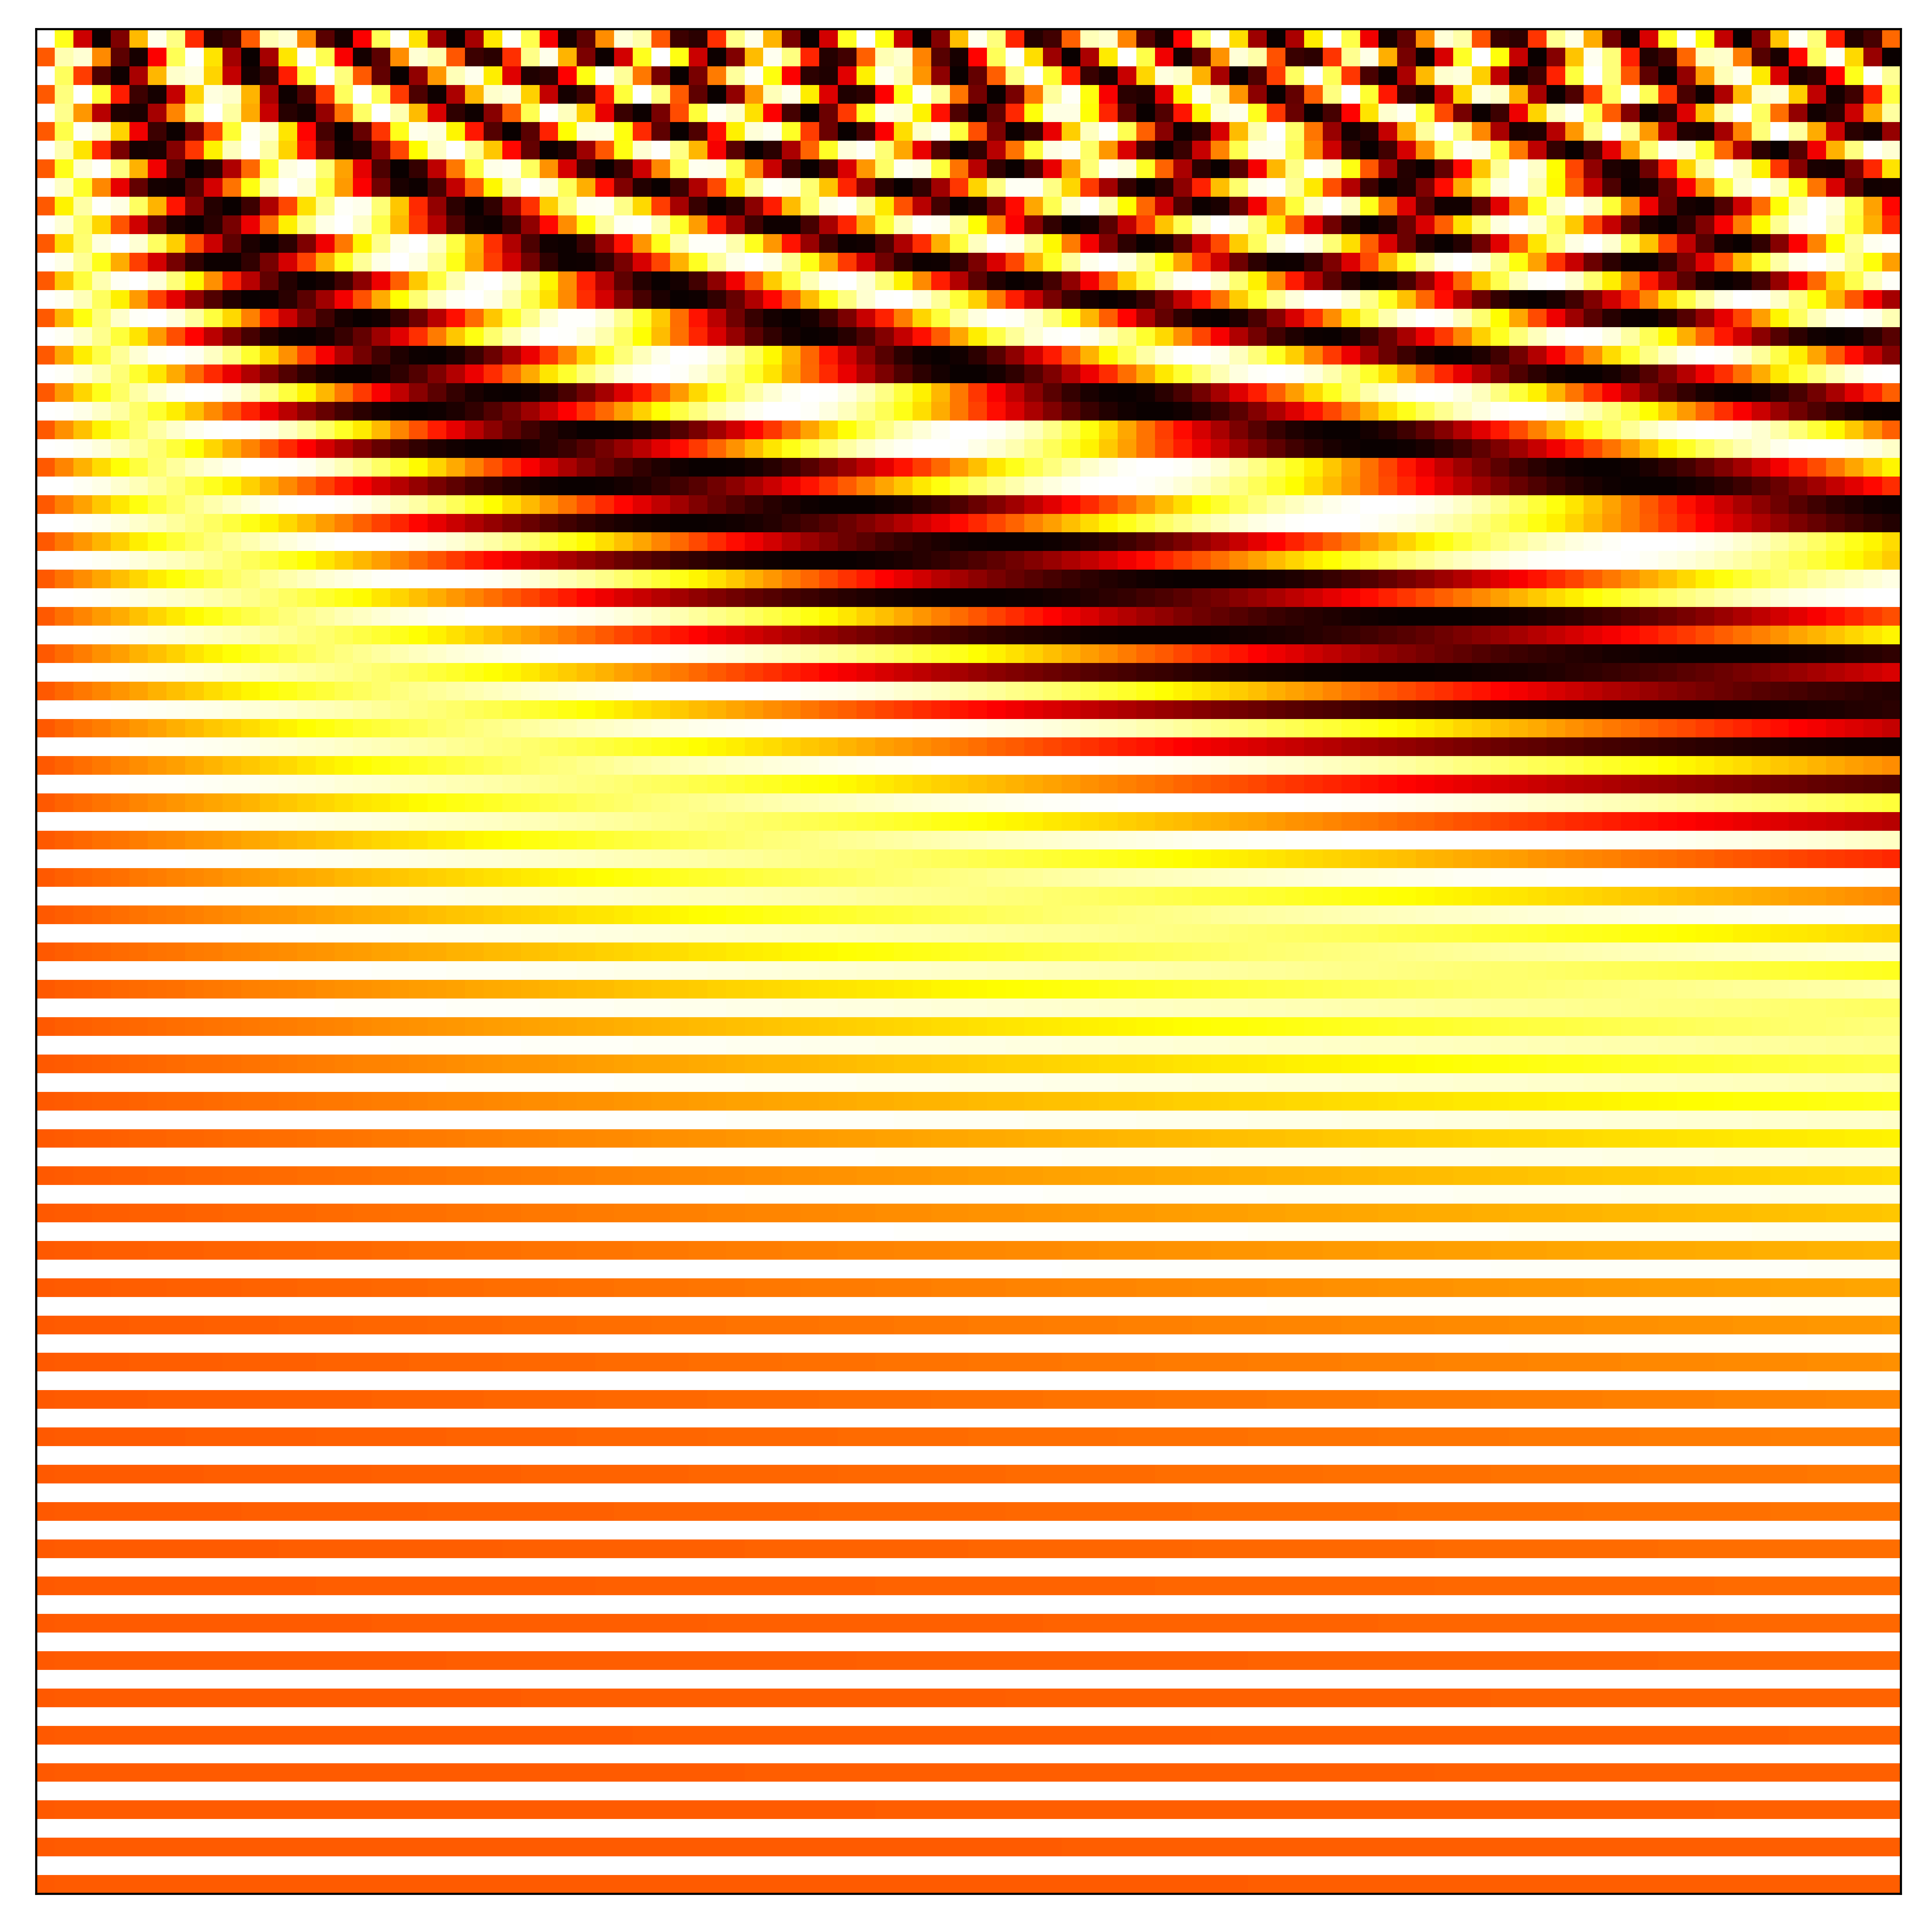
\includegraphics[scale=\myscale,scale=0.4]{figures/position-matrix}
\end{center}


%--------------------------------------------------------------------
\subsection{Positions relatives}

Ce qui est important pour la compréhension d'une phrase, c'est la position des mots/tokens les uns par rapport aux autres. Étant donnés deux vecteurs position $w$ et $w'$, il faut donc que le réseau puisse trouver rapidement leurs positions relatives et donc que la transformation qui envoie un vecteur position sur un autre soit simple afin de pouvoir être facilement obtenue lors de l'apprentissage.
Nous allons voir que la transformation $w_k \mapsto w_{k+1}$ d'un vecteur position à la position suivante se fait simplement par multiplication d'une matrice :
$w_{k+1} = R_1 w_k$ où $R_1 \in M_{n,n}$ est une matrice (indépendante de $k$).

Notons $M(\omega) \in M_{2,2}$ la matrice de la rotation du plan d'angle $\omega$ (centrée à l'origine) :
\[
M(\omega) = 
\begin{pmatrix}
	\cos(\omega) & -\sin(\omega) \\
	\sin(\omega) & \cos(\omega)
\end{pmatrix}
\]	
Appliquer $\ell$ rotations d'angle $\omega$ revient à effectuer une rotation d'angle $\ell\omega$, ainsi $M(\omega)^\ell = M(\ell\omega)$.

\myfigure{0.8}{
	\tikzinput{position-02}
} 


Notons $R_1 \in M_{n,n}$ la matrice diagonale par bloc :

\[
R_1 = 
\begin{pmatrix}
	M(\omega_0) & && \\ 
	& M(\omega_1) & &  \\
	& & \ddots &  \\
	& & & M(\omega_{n/2-1}) \\ 			
\end{pmatrix}
\quad \text{ et } \quad
R_\ell = R_1^\ell = 
\begin{pmatrix}
	M(\ell\omega_0) & && \\ 
	& M(\ell\omega_1) & &  \\
	& & \ddots &  \\
	& & & M(\ell\omega_{n/2-1}) \\ 			
\end{pmatrix}
\]

\begin{proposition}
\sauteligne
\begin{itemize}	
  \item $w_{k+1} = R_1 w_k$	quel que soit $k$,
  \item $w_{k+\ell} = R_\ell w_k$ quel que soit $k$.
\end{itemize}
\end{proposition}

La preuve est simplement l'application des formules d'addition de $\cos(a+b)$ et $\sin(a+b)$.

Conclusion : passer d'un vecteur position à la position suivante correspond à la multiplication par la matrice $R_1$. Passer à une position plus éloignée correspond à la multiplication par une matrice $R_\ell$. C'est donc une transformation suffisamment simple pour que réseau la retrouve tout seul lors de l'apprentissage.


%%%%%%%%%%%%%%%%%%%%%%%%%%%%%%%%%%%%%%%%%%%%%%%%%%%%%%%%%%%%%%%%%%%%%
\section{Produit tensoriel}

Un produit tensoriel de type $(1,1)$ envoie linéairement un vecteur $X$ sur un vecteur $Y$, cela correspond à l'action d'une matrice: $Y = AX$.
L'attention, qui est à la base de ce chapitre, est fondée sur le produit tensoriel de type $(2,2)$: une matrice est transformée en une autre matrice.

%--------------------------------------------------------------------
\subsection{Action du produit tensoriel}

Considérons deux matrices $A \in M_{p,p}$ (carrée de taille $p$) et $B \in M_{n,n}$ (carrée de taille $n$).
L'action du \defi{produit tensoriel} $A \otimes B$ sur une matrice $M \in M_{n,p}$ ($n$ lignes et $p$ colonnes) est définie par :
\mybox{$(A \otimes B) M = B M A^T$}
Ainsi le produit tensoriel $A \otimes B$ transforme une matrice $M \in M_{n,p}$ en une matrice $M' =B M A^T \in M_{n,p}$ de même taille.
On rappelle que si $A = (a_{ij})_{1 \le i,j \le p}$ alors sa transposée est $A^T = (a_{ji})_{1 \le i,j \le p}$.

\bigskip

\textbf{Développement partiel.}

Notons la matrice $M = (C_1, C_2, \ldots, C_p)$ sous la forme de ses $p$ vecteurs colonnes.
Notons $A = (a_{ij})_{1 \le i,j \le p}$ les coefficients de $A$.
Notons la matrice $M' = (A \otimes B) M = BMA^T$ et écrivons $M' = (C'_1, \ldots, C'_p)$ sous la forme de ses vecteurs colonnes.
Alors, pour $1 \le j \le p$: 

\begin{equation}
	\label{eq:produittensoriel}
	\tag{\dag}
	C'_j = \sum_{i=1}^p a_{ij} BC_i.
\end{equation}



\begin{exemple}
	Soient
$$A = 
\begin{pmatrix}
1 & 2 \\ 
3 & 4 \\
\end{pmatrix},
\qquad
B = 
\begin{pmatrix}
2 & -1 \\
1 & 0 \\
\end{pmatrix},
\qquad
M = 
\begin{pmatrix}
1 & 2 \\
0 & 1 \\
\end{pmatrix}.
$$
Alors 
$$
M' = (A \otimes B) M = BMA^T = 
\begin{pmatrix}
	2 & -1 \\
	1 & 0 \\
\end{pmatrix}
\begin{pmatrix}
	1 & 2 \\
	0 & 1 \\
\end{pmatrix}
\begin{pmatrix}
	1 & 3 \\ 
	2 & 4 \\
\end{pmatrix}
=
\begin{pmatrix}
	8 & 18 \\ 
	5 & 11 \\
\end{pmatrix}.
$$
\end{exemple}

\bigskip

\textbf{Interprétation.}

\begin{itemize}
	\item Notons de nouveau $M = (C_1, C_2, \ldots, C_p)$ sous la forme de $p$ vecteurs colonnes.
	Soit $a = \left(\begin{smallmatrix} a_1 \\ \vdots \\ a_p \end{smallmatrix}\right)$ un vecteur colonne. Alors le produit $Ma$ correspond à une combinaison linéaire de ses vecteurs colonnes :
	$$ Ma = \sum_{j = 1}^p a_j C_j.$$
	Ainsi, multiplier la matrice $M$ par la droite revient à une action sur les colonnes de $M$.
	Dans le contexte de l'attention, l'indice $j=1,\ldots,k$ correspond à  la position d'un token ; 
	ainsi la multiplication à droite de $M$ par $A^T$ correspond à une \emph{action sur les positions} des tokens.
		
	\item Considérons maintenant la même matrice comme étant la superposition de $n$ lignes $L_1,\ldots,L_n$.
	Soit $b = (b_1,\ldots,b_n)$ un vecteur ligne. Le produit $bM$ correspond à une combinaison linéaire des lignes de $M$ :
	$$bM = \sum_{i=1}^{n} b_i L_i.$$
	Ainsi, multiplier $M$ par la gauche correspond à une action sur les lignes.
	Autrement dit, chaque vecteur colonne reste à sa place, mais ses coefficients sont transformés.
	Dans notre contexte cela signifie que les positions sont inchangées mais que l'on change le plongement de chaque vecteur token, on parle d'\emph{action sur la dimension}.
	
	\item Le produit tensoriel combine ces deux actions !
	
\end{itemize}

Remarque : dans notre situation, les coefficients de $A$ et $B$ seront déterminés par apprentissage, donc la transposition dans la formule $B M A^T$ est inutile d'un point de vue pratique.

%--------------------------------------------------------------------
\subsection{Propriétés}

\begin{itemize} 
	\item \textbf{Linéarité à gauche et à droite.}
Le produit tensoriel est linéaire à gauche et linéaire à droite (il est donc bilinéaire), en particulier :
$$(A_1 + A_2) \otimes B =  (A_1 \otimes B) + (A_2 \otimes B)$$
$$ A \otimes (B_1 + B_2) =  (A \otimes B_1) + (A \otimes B_2)$$

Plus précisément, la première égalité signifie que $\big(( A_1 + A_1) \otimes B\big) M =  (A_1 \otimes B)M + (A_2 \otimes B) M$.

   \item \textbf{Formule du produit.}
   Le produit tensoriel vérifie la formule du produit :
   $$(A_1 \otimes B_1) \times (A_2 \otimes B_2) = (A_1 A_2) \otimes (B_1 B_2)$$
   Ici \og{}$\times$\fg{} désigne le produit usuel de matrices.
   
   \item On a les formules $(I \otimes B)M = BM$ et $(A \otimes I)M = MA^T$ où $I$ désigne une matrice identité (de taille adéquate), ainsi par la formule du produit :
   $$ (A \otimes B)(M) = (I \otimes B) \times (A \otimes I) (M).$$
	
\end{itemize}

Le produit tensoriel est exactement l'outil qui permet de regrouper une action sur les vecteurs colonnes (via la matrice $A$) avec une action sur les vecteurs lignes (via la matrice $B$).


Toutes ces formules se vérifient facilement en utilisant la définition $(A \otimes B) M = BMA^T$ (et en se souvenant que $(A_1A_2)^T = A_2^T A_1^T$).   


%--------------------------------------------------------------------
\subsection{Produit de Kronecker}

Jusqu'ici nous n'avons pas vraiment défini ce qu'est $A \otimes B$, car nous avons juste décrit ce qu'est l'action de $A \otimes B$ sur une matrice $M$.
Une façon directe de définir $A \otimes B$ est de le faire via le \defi{produit de Kronecker} comme une (grande) matrice carrée avec $np$ lignes et $np$ colonnes.

$$A \otimes B = 
\begin{pmatrix} 
a_{11}B & a_{12}B & \dots  & a_{1p}B \\
a_{21}B & A_{22}B & \dots  & a_{2p}B \\
\vdots  & \vdots  & \vdots & \ddots  \\
a_{p1}B & \dots   & \dots  & a_{pp}B
\end{pmatrix}
\in M_{np,np}	
$$

Dans cette écriture, chaque élément est en fait la matrice $B$ multipliée par un coefficient $a_{ij}$. 

Pour appliquer cette version du produit tensoriel à une matrice $M$, il faut d'abord la vectoriser.
Si $M = (C_1, C_2, \ldots, C_p) \in M_{n,p}$ est écrite sous forme de vecteurs colonnes, alors $\operatorname{vec(M)}$ est le vecteur obtenu en superposant tous ses vecteurs colonnes :
$$\operatorname{vec}(M) = \begin{pmatrix} C_1 \\ C_2 \\ \vdots \\ C_p \end{pmatrix}$$

Modulo cette vectorisation et en calculant le produit $\operatorname{vec}(M)$ par la grande matrice $A \otimes B$ on retrouve bien la formule \eqref{eq:produittensoriel} précédente, c'est-à-dire :
$$(A \otimes B) \operatorname{vec}(M) = \operatorname{vec}(B M A^T).$$

\begin{exemple}
Reprenons l'exemple précédent avec :
$$A = 
\begin{pmatrix}
	1 & 2 \\ 
	3 & 4 \\
\end{pmatrix},
\qquad
B = 
\begin{pmatrix}
	2 & -1 \\
	1 & 0 \\
\end{pmatrix},
\qquad
M = 
\begin{pmatrix}
	1 & 2 \\
	0 & 1 \\
\end{pmatrix}.
$$

Alors 

\[
A \otimes B
\begin{pmatrix}
	1\begin{bmatrix}	2 & -1 \\1 & 0 \\\end{bmatrix}   & 
	2\begin{bmatrix}	2 & -1 \\1 & 0 \\\end{bmatrix}   \\	 
	3\begin{bmatrix}	2 & -1 \\1 & 0 \\\end{bmatrix}   & 
    4\begin{bmatrix}	2 & -1 \\1 & 0 \\\end{bmatrix}   \\	 	
\end{pmatrix}
= 
\begin{pmatrix}
2 & -1 & 4 & -2 \\
1 &  0 & 2 & 0 \\
6 & -3 & 8 & -4 \\
3 & 0 & 4 & 0 \\	
\end{pmatrix},
\qquad 	
\operatorname{vec}(M) 
= \begin{pmatrix} 1 \\ 0 \\ 2 \\ 1 \end{pmatrix},
\qquad 
(A \otimes B) \operatorname{vec}(M) 
= \begin{pmatrix} 8 \\ 5 \\ 18 \\ 11 \end{pmatrix}.
\]
Donc après remise en forme du vecteur $(A \otimes B) \operatorname{vec}(M)$ sous forme d'une matrice, on retrouve 
$$
(A \otimes B) M = 
\begin{pmatrix}
	8 & 18 \\ 
	5 & 11 \\
\end{pmatrix}.
$$
\end{exemple}



%%%%%%%%%%%%%%%%%%%%%%%%%%%%%%%%%%%%%%%%%%%%%%%%%%%%%%%%%%%%%%%%%%%%%
\section{Attention}

%--------------------------------------------------------------------
\subsection{Tri-grammes à trou}

Rappelons que l'objectif est de compléter le début d'une phrase en déterminant le mot suivant le plus probable, puis en itérant le processus.
Dans le chapitre précédent nous avons vu qu'en calculant les occurrences des bi-grammes (mot1, mot2), on complétait une phrase se terminant par mot1 en choisissant mot2 de telle sorte que le bi-gramme (mot1, mot2) soit le plus fréquent parmi tous les bi-grammes (mot1, autre mot).
On peut améliorer la technique en comptant les occurrences de tri-grammes (mot1, mot2, mot3) et cette fois une phrase se terminant par (mot1, mot2) sera complétée par le mot3 le plus probable.

Cependant regarder seulement les tous derniers mots d'une phrase n'est pas suffisant pour la comprendre. Bien souvent le contexte de la phrase est donné bien avant dans le texte.
Nous allons considérer les \defi{tri-grammes à trou} :
\mycenterline{ (mot1, \trou, mot2, mot3).}
Le mot1 joue le rôle du contexte, le mot2 sera le dernier mot de notre phrase à compléter et le mot3 sera le mot par lequel la phrase sera complétée. Entre mot1 et mot2, il peut y avoir plusieurs mots dont on ne tient pas compte.

\begin{exemple}
On veut comprendre le mot2 = \mot{signer}, dernier mot d'un texte à compléter.

Si on trouve le mot \mot{appartement} (qui joue le rôle du mot1) auparavant dans le texte alors voici différente propositions pour compléter la phrase :
\mycenterline{ \mot{appartement} \trou \mot{signer} 
\begin{tabular}{|l}
	\mot{le bail} \\
	\mot{le contrat} \\	
	\mot{l'offre} \\	
\end{tabular}
}

Mais si auparavant dans le texte on avait trouvé le terme \mot{guerre} ou bien \mot{Picasso} alors le contexte serait différent, donc la complétion aussi.
\mycenterline{ \mot{guerre} \trou \mot{signer} 
	\begin{tabular}{|l}
		\mot{la paix} \\
		\mot{l'armistice} \\	
		\mot{la déclaration} \\	
	\end{tabular}
}

\mycenterline{ \mot{Picasso} \trou \mot{signer} 
	\begin{tabular}{|l}
		\mot{le tableau} \\
		\mot{la peinture} \\	
		\mot{l'\oe uvre} \\	
	\end{tabular}
}


\end{exemple}

Remarque : pour nos explications nous inclurons l'article dans le mot, ainsi \mot{le chat} est considéré comme un seul mot.

Ce processus de tri-grammes à trous est très efficace, surtout dans les situations pas très subtiles où il s'agit essentiellement de faire de la copie (par exemple dans du code informatique où il y a beaucoup de structures qui se répètent).

Par exemple :
 \mycenterline{ \mot{grand} \trou \mot{très} 
 	\begin{tabular}{|l}
 		\mot{grand} \\
 		\mot{petit} \\	
 	\end{tabular}
 }

 \mycenterline{ \mot{deux} \trou \mot{un}, 
	\begin{tabular}{|l}
		\mot{deux} \\
	\end{tabular}
}

Bien évidemment, la difficulté est de déterminer le contexte. Plus précisément, 
quel est le mot1 le plus pertinent qui donne à mot2 son sens dans la phrase ?
C'est là que le concept d'attention joue son rôle.
Considérons une phrase à compléter :
\mycenterline{mot1, mot2, mot3, \ldots, mot$n$}
L'attention va attribuer à chacun de ces mots une probabilité selon son importance dans la signification de la phrase.

\begin{exemple}
Considérons le début de phrase :
	\mycenterline{\mot{ Le petit chat noir mange \ldots}}
L'attention attribue une valeur d'intérêt à chaque mot :

\begin{center}
\begin{tabular}{cccc}
	\mot{le petit} & \mot{chat} & \mot{noir} & \mot{mange} \\
	5\% & 40\% & 5\% & 50\% \\  
\end{tabular} 
\end{center}

Ainsi les deux mots importants sont \mot{chat} et \mot{mange}, et on compléterait naturellement la phrase par \mot{souris} (ou \mot{croquettes}) sans se préoccuper des termes \mot{petit} ou \mot{noir}.
Remarquer qu'ici l'attention a mis en évidence le sujet et le verbe. Ces règles ne sont pas expliquées au réseau de neurones mais apprises par assimilation d'un grand corpus.	
\end{exemple}
	
	
%--------------------------------------------------------------------
\subsection{Principe de l'attention}

L'attention est définie par un produit tensoriel et envoie une matrice $M \in M_{r,K}$ ($r$ lignes, $K$ colonnes) sur une autre matrice $h(M) \in M_{r,K}$ de même taille, via l'opération :
$$h(M) = (A \otimes B) M$$
où $A \in M_{K,K}$ et $B \in M_{r,r}$.

\begin{itemize}
	\item $K$ est le nombre de tokens pris en compte, c'est-à-dire la longueur de la phrase à compléter ($K = 1024$ pour \emph{GPT2}).
	
	\item $A \in M_{K,K}$ est la matrice d'attention, ses coefficients sont calculés via des poids du réseau de neurones (par une formule un peu compliquée qu'on expliquera plus tard).
	
	\item $r$ est la dimension de l'espace de travail, c'est un diviseur de $n$ la dimension de plongement ($r=64$, $n=768$ pour \emph{GPT2}).
	
	\item $B \in M_{r,r}$ est une matrice de plongement.
	
	\item $M \in M_{r,K}$ est une matrice dont chaque colonne $w_k \in \Rr^r$ correspond à une partie du vecteur token $v_k \in \Rr^n$.
	
	\item $n/r$ est le nombre de têtes d'attention (\emph{attention head}), c'est-à-dire le nombre de fonctions $h$ que l'on va construire à chaque couche d'attention ($n/r = 768/64 = 12$ pour \emph{GPT2}).
\end{itemize}

Quel est l'intérêt du nouveau paramètre $r$ ? 
Une tête d'attention $h$ ne travaille pas sur tout l'espace $\Rr^n$ des vecteurs tokens mais seulement sur un sous-espace de celui-ci. On a vu que travailler avec des sous-espaces permet de transmettre de l'information directe d'une couche à une autre via le flux résiduel.
De plus, une tête d'attention, une fois entraînée, se spécialise pour une fonction (copie d'un terme, détection des positions,...). La couche d'attention regroupe plusieurs têtes d'attention travaillant en parallèle (\emph{multi-head attention}). Le nombre de têtes d'attention (par couche) étant $n/r$ et chacune travaillant sur un espace de dimension $r$, une couche d'attention travaille bien sur un espace de dimension totale $n$, qui correspond à notre dimension de l'espace $\Rr^n$ des vecteurs tokens.

Avec plusieurs têtes d'attention $h_1,h_2,\ldots,h_{n/r}$ on calcule la sortie par l'opération :
$$x_{i+1} = x_i \ + \ \sum_{j=1}^{n/r} W_{\text{out}}^{(j)} \cdot h_j \cdot  W_{\text{in}}^{(j)} \cdot x_i$$
où $W_{\text{in}}^{(j)} \in M_{r,n}$, $W_{\text{out}}^{(j)} \in M_{n,r}$ (pour $j=1,\ldots,n/r$) (ces matrices dépendent aussi de la couche numéro $i$).

\myfigure{0.8}{
	\tikzinput{attention-01}
} 

Une autre façon de faire (équivalente) serait de concaténer les fonctions $h_i$ par des sommes directes, afin de définir $H \in M_{n,n}$ par 
$H = h_1 \oplus h_2 \oplus \cdots \oplus h_{n/r}$, c'est-à-dire $H$ est la matrice diagonale par bloc :
$$H = \begin{pmatrix}
	h_1 & && \\ 
	& h_2 & &  \\
	& & \ddots &  \\
	& & & h_{n/r} \\ 			
\end{pmatrix}$$
Puis de calculer 
$$x_{i+1} = x_i \ + \ W_{\text{out}}\cdot H \cdot W_{\text{in}} \cdot x_i$$
où $W_{\text{in}} \in M_{n,n}$, $W_{\text{out}} \in M_{n,n}$.
	

Il nous reste maintenant à expliquer comment est définie la matrice d'attention $A \in M_{K,K}$.
Les coefficients de $A$ ne sont pas directement des poids du réseau, pour $K = 1024$ cela ferait plus d'un million de poids supplémentaires par matrice d'attention (et il y $12 \times 12$ têtes d'attention avec \emph{GPT2}). Nous allons définir plus efficacement $A$ via un produit de matrices de taille $r\times n$ afin d'obtenir un nombre de poids de l'ordre de $rn = 65\,536$.


%--------------------------------------------------------------------
\subsection{Formule de l'attention}

Donnons maintenant la formule exacte de l'attention issue de l'article fondateur \emph{Attention is all you need} d'une équipe de \emph{Google} à la base du modèle \emph{GPT2} et de tous ses successeurs.
Nous allons suivre la formalisation de l'article \emph{A mathematical framework for transformer circuits}. La construction reste assez technique et les notations nombreuses.
Pour ces explications nous allons suivre les notations des articles cités et de la littérature ; il y aura donc des petites différences avec les sections précédentes. Cependant, on choisit ici une convention mathématique : on considère les vecteurs tokens comme des vecteurs colonnes, ainsi dans la matrice $x_i$ du flux résiduel, chaque vecteur colonne correspond à un vecteur token (la convention usuelle est que les vecteurs tokens sont les lignes de cette matrice).

\bigskip

\textbf{Les têtes d'attention.}

On se place à la couche numéro $i$, supposée une couche d'attention.
On récupère du flux résiduel une matrice $x_i \in M_{n,K}$ 
%($n$ lignes, $K$ colonnes),
dont les vecteurs colonnes sont les $K$ vecteurs tokens.
Après cette couche, le flux résiduel est :
$$x_{i+1} = x_i + H_i ( x_i )$$
où $H_i$ est une transformation qui transforme une matrice de $M_{n,K}$ en une matrice de même taille ($H_i$ dépend de la couche de $i$ et n'est pas tout à fait le même que le $H$ de la section précédente puisque il va inclure ici les matrices de plongement).
L'attention globale $H_i$ est en fait la somme de têtes d'attention $h \in \mathcal{H}_i$ de cette couche :
$$H (x_i)  = \sum_{h \in \mathcal{H}_i} h (x_i) $$

Chaque tête d'attention est définie par un produit tensoriel :
$$h(x) = \big(A^{[h]} \otimes W^{[h]}_{OV} \big) x_i,$$
où $A^{[h]} \in M_{K,K}$ et $W^{[h]}_{OV} \in M_{n,n}$.
L'exposant $[h]$ indique que ces matrices dépendent de la tête d'attention $h$. Comme dans la suite on ne va considérer qu'une seule tête d'attention $h$, on ne précise plus cette dépendance et on écrira simplement :
$$h(x) = \big(A \otimes W_{OV} \big) x_i$$

\bigskip

\textbf{Décomposition d'une tête d'attention.}

On s'intéresse à une tête d'attention $h$.
On note $W_V \in M_{r,n}$ et $W_O \in M_{r,n}$, alors $W_{OV} \in M_{n,n}$ est définie par 
$$W_{OV} = W_O \times W_V.$$
On note de nouveau $A \in M_{K,K}$ la matrice d'attention, alors par la formule du produit :
\[
A \otimes W_{OV} = A \otimes (W_O W_V) = 
(\underbrace{W_O \otimes I}_{\text{écriture}}) \cdot 
(\underbrace{A \otimes I}_{\text{attention}}) \cdot (\underbrace{I \otimes W_V}_{\text{lecture}})
\]
Cette écriture décompose le travail :
\begin{itemize}
	\item La matrice $W_V$ ($V$ pour \emph{Values}) lit $x_i$ sur le flux résiduel et transforme $x_i \mapsto W_V x_i$  via un plongement linéaire dans un espace $\Rr^r$. Autrement dit, chaque vecteur token (de taille $n$) est lu et transformé mais en ne retenant que $r$ dimensions.
	
	\item Ensuite intervient le mécanisme d'attention via la matrice $A$ qui correspond à une action sur les colonnes des vecteurs tokens. La matrice $A$ va mettre en évidence les mots/tokens les plus significatifs pour un mot/token donné.
	
	\item La matrice $W_O$ ($O$ pour \emph{Output}) plonge un vecteur de $\Rr^r$ en un vecteur de $\Rr^n$ qui sera ajouté au flux résiduel.
\end{itemize}

Les coefficients de $W_V$ et $W_O$ sont des poids du réseau.
Même si la matrice $W_{OV}$ est de taille $n \times n$, ses $n^2$ coefficients ne sont pas directement les poids du réseau, en effet elle est définie par le produit de deux matrices de taille $r \times n$ et $n \times r$ (donc avec seulement $2rn$ coefficients), c'est donc une matrice de rang faible (on rappelle que $\operatorname{rg}(AB) \le \min( \operatorname{rg}(A) ,\operatorname{rg}(B) )$).


\bigskip

\textbf{Formule pour l'attention $A$.}

L'action de l'attention est définie par :
$$(A \otimes I) x = \operatorname{softmax} \big( x^T W_Q^T W_K^T x \big)$$
où 
\begin{itemize}
	\item $x \in M_{n,K}$ est la matrice dont les colonnes sont des vecteurs tokens,
	\item $W_K, W_Q \in M_{r,n}$ ($K$ pour \emph{Keys}, $Q$ pour \emph{Queries}) sont des matrices de plongement (qui transforment un vecteur de $\Rr^n$ en un vecteur de $\Rr^r$). Les coefficients de ces deux matrices sont des poids du réseau.
	\item $x^T$ et $W_Q^T$ désigne la transposition de $x$ et $W_Q$.
	\item $\operatorname{softmax}(M)$ désigne la fonction softmax $\sigma$ appliquée à chacune des lignes de la matrice $M$. Ainsi chaque ligne de la matrice $M$ est interprétée comme une liste de probabilités, mettant en évidence les mots/tokens les plus importants.
	
\end{itemize}


On note souvent $K = W_K x \in M_{r,K}$ et $Q = W_Q x \in M_{r,K}$ les matrices des clés et des requêtes, qui contiennent, en colonnes, des morceaux de vecteurs tokens plongés.
Le point important est que ces deux plongements sont différents et vont permettre de comparer les mots/tokens d'une phrase entre eux.
L'attention s'écrit alors
$$(A \otimes I) x = \operatorname{softmax} \big( Q^T K \big)$$

Remarque : comme au fil des couches les coefficients ont tendance à grossir, dans la formule de l'article original, on divise par un terme $\sqrt{r}$ (où $r$ est la dimension du petit espace ambiant) : 
$$(A \otimes I) x = \operatorname{softmax} \left( \frac{Q^T K}{\sqrt r} \right)$$


%--------------------------------------------------------------------
\subsection{Auto-attention}

On se concentre maintenant uniquement sur les explications de la formule de l'attention $A$.


\textbf{Produit scalaire.}

On souhaite comparer deux mots entre eux et attribuer (par apprentissage) une valeur de pertinence du mot1 vis à vis du mot2. Considérons un premier mot, mot1, défini par un vecteur $q \in E_Q = \Rr^r$. On peut considérer $q$ comme un morceau d'un vecteur token de $\Rr^n$.
Considérons un second mot, mot2, défini par un vecteur $k \in E_K = \Rr^r$.
De nouveau $k$ est considéré comme un morceau d'un vecteur token de $\Rr^n$.
On compare ces deux vecteurs $q$ et $k$ en calculant le produit scalaire $\langle q \mid k \rangle$.
Si on considère $q$ et $k$ comme des vecteurs colonnes alors $q^T$ désigne le vecteur ligne et le produit scalaire est égal au produit de matrices :
$$\langle q \mid k \rangle = q^T \times k$$

Note : on pourrait aussi comparer les deux vecteurs via la similarité cosinus ce qui est presque équivalent.


\begin{exemple}
On souhaite comparer le mot \mot{château} et \mot{princesse}.
Au préalable on transforme le mot \mot{château} en un vecteur token $v_{\text{château}} \in \Rr^n$,
on calcule ensuite un vecteur requête : 
$$q = W_Q v_{\text{château}} \in E_Q = \Rr^r.$$
Ensuite, on transforme le mot \mot{princesse} en un vecteur token $v_{\text{princesse}} \in \Rr^n$,
on calcule ensuite un vecteur clé : 
$$k = W_K v_{\text{princesse}} \in E_K = \Rr^r.$$
Supposons qu'après calculs (avec $r=4$) :
$$
q = \begin{pmatrix} 2 \\ 1 \\ 4 \\ 3 \end{pmatrix} \in \Rr^4
\qquad
k =  \begin{pmatrix} -1 \\ 3 \\ 0 \\ 2 \end{pmatrix} \in \Rr^4
$$
Alors 
$$
\langle q \mid k \rangle = q^T k = 
\begin{pmatrix} 2 & 1 & 4 & 3 \end{pmatrix}
\begin{pmatrix} -1 \\ 3 \\ 0 \\ 2 \end{pmatrix}
= 2 \times (-1) + 1 \times 3 + 4 \times 0 + 3 \times 2 = 7 
$$
Il est important de comprendre que même si $q$ et $k$ sont des vecteurs de même taille, ils n'ont pas été plongés de la même façon dans $\Rr^r$, c'est pourquoi on distingue $E_Q$ de $E_K$ même s'ils sont tous les deux égaux à $\Rr^r$.

Ainsi on peut comparer le mot \mot{château} avec lui même ! 
On considère le même $q = W_Q v_{\text{château}} \in E_Q$.
Par contre si on calcule $k = W_K v_{\text{château}} \in E_Q$, il n'y a aucune raison que $q$ et $k$ soit égaux si $W_Q$ et $W_K$ sont distinctes.
Supposons par exemple 
$$
k =  \begin{pmatrix} -2 \\ 0 \\ 2 \\ 2 \end{pmatrix} \in \Rr^4
$$
Alors cette fois :
$$
\langle q \mid k \rangle = q^T k = 10
$$
\end{exemple}

\bigskip

\textbf{Un exemple d'attention.}

Considérons la phrase :

\mycenterline{\mot{Jeanne visite le zoo, émerveillée}}

Pour nos explications cette phrase se décompose en quatre tokens \mot{Jeanne}, \mot{visite},
\mot{le zoo}, \mot{émerveillée}. 
%Normalement \mot{un} et \mot{le} devrait être des tokens à part, mais il serait attribué de coefficient d'attentiv_{\text{\mot{Jeanne}}}on proche de $0$.

Une fois entraîné, le réseau calcule quatre vecteurs tokens par plongement initial,
$v_1 =  v_{\text{\mot{Jeanne}}}$, $v_2 = v_{\text{\mot{visite}}}$, $v_3$, $v_4$.
La juxtaposition de ces quatre vecteurs colonnes, forme la matrice $x_1$ du flux résiduel :
$$x_ 1 = \big( 
v_{\text{\mot{Jeanne}}},
v_{\text{\mot{visite}}}, 
v_{\text{\mot{zoo}}},
v_{\text{\mot{émerveillée}}} \big).$$
Le but est de remplacer chacun de ces vecteurs par une combinaison linéaire des vecteurs expliquant le mieux le mot concerné et d'écrire la matrice résultante sur le flux résiduel :
$$x_2 = \big(w_1, w_2, w_3, w_4\big)$$
Par exemple, quels mots dans cette phrase se rattachent le plus au mot \mot{zoo} ?
Il y a bien sûr le mot \mot{zoo} lui même, mais aussi \mot{visite}, les autre mots étant beaucoup moins significatifs. Ainsi on pourrait avoir 
$$w_3 = 
0.1 \, v_{\text{\mot{Jeanne}}}
+ 0.4 \,v_{\text{\mot{visite}}}
+ 0.4\, v_{\text{\mot{zoo}}}
+0.1\, v_{\text{\mot{émerveillée}}}
$$
Il faut faire le même travail pour les autres mots, par exemple $w_4$ est le vecteur expliquant le mot \mot{émerveillée} qui se rattache surtout à \mot{Jeanne} (et un peu à \mot{zoo}), on pourrait donc avoir :
$$w_4 = 
0.3 \,v_{\text{\mot{Jeanne}}}
+ 0.0\, v_{\text{\mot{visite}}}
+ 0.2\, v_{\text{\mot{zoo}}}
+0.5\, v_{\text{\mot{émerveillée}}}
$$


Voyons comment notre tête d'attention $h$ calcule les poids définissant les vecteurs $w_i$.
Via les deux matrices de plongement, on calcule les vecteurs requêtes et les vecteurs clés $(1 \le i \le 4$) :
$$q_i =  W_Q v_i \qquad \text{ et } \qquad k_i =  W_K v_i$$

\myfigure{0.5}{\small
	\tikzinput{attention-02}
} 

Pour le mot numéro $1$, \mot{Jeanne}, on calcule le produit scalaire de $q_1$ avec chaque $k_j$ pour $j=1,\ldots,4$.
$$\alpha_j = \langle q_1 \mid k_j \rangle = q_1^T k_1$$
puis on applique la fonction softmax $\sigma$ pour obtenir 
$$(\gamma_1, \gamma_2, \gamma_3, \gamma_4)  = \sigma(\alpha_1, \alpha_2, \alpha_3, \alpha_4)$$
qui vérifient $\gamma_1 + \gamma_2 + \gamma_3 + \gamma_4 = 1$.
Ces coefficients $\gamma_i$ sont les poids des vecteurs $v_i$ pour comprendre le mot numéro $1$ :
$$w_1 = \alpha_1 v_1 + \alpha_2 v_2 + \alpha_3 v_3 + \alpha_4 v_4.$$
Par exemple :
$$w_1 = 0.2 v_1 + 0.4 v_2 + 0.1 v_3 + 0.3 v_4.$$ 
C'est-à-dire :
$$w_{\text{\mot{Jeanne}}} = 0.2 v_{\text{\mot{Jeanne}}} + 0.4 v_{\text{\mot{visite}}} + 0.1 v_{\text{\mot{zoo}}} + 0.3 v_{\text{\mot{émerveillée}}}.$$ 

%Bien sûr au fil des couches, il n'est plus clair que le premier vecteur corresponde au premier mot.

Il faut refaire ces opérations pour les mots suivants afin d'obtenir $x_2 = (w_1, w_2, w_3, w_4)$.

Par exemple $q_2^T k_j$ correspond aux poids expliquant le mot \mot{visite}, on pourrait avoir :
$$w_3 = 0.2 v_1 + 0.4 v_2 + 0.4 v_3 + 0.0 v_4.$$ 

\begin{center}
\begin{tabular}{l|ccccc}
      &   & \mot{Jeanne} & \mot{visite} & \mot{zoo} & \mot{émerveillée} \\	
                  &       & $k_1$ & $k_2$ & $k_3$ & $k_4$  \\ \hline	                  
\mot{Jeanne}      & $q_1$ & 0.2 & 0.4 & 0.1 & 0.3 \\
\mot{visite}      & $q_2$ & 0.1 & 0.4 & 0.4 & 0.1 \\
\mot{zoo}         & $q_3$ & 0.2 & 0.4 & 0.4 & 0.0 \\
\mot{émerveillée} & $q_4$ & 0.1 & 0.4 & 0.4 & 0.1 \\	
\end{tabular}	
\end{center}

Ces calculs sont condensés dans la formule matricielle de l'attention :
$$h(x_1) = \operatorname{softmax} \big( Q^T K \big)$$
où $Q = W_Q x_1$ et $K = W_K x_1$.

Ainsi la matrice $h(x_1)$ est composée, ligne par ligne, des coefficients précédents :
$$h(x_1) = 
\begin{pmatrix}
0.2 & 0.4 & 0.1 & 0.3 \\
0.1 & 0.4 & 0.4 & 0.1 \\
0.2 & 0.4 & 0.4 & 0.0 \\
0.1 & 0.4 & 0.4 & 0.1 \\
\end{pmatrix}
$$


%--------------------------------------------------------------------
\subsection{Exemple de \emph{GPT2}}

Considérons la phrase \mot{The dog is black} constituée des tokens \mot{The}, \mot{␣dog}, \mot{␣is}, \mot{␣black}.
Calculons la matrice d'attention $h$ associée à la couche d'attention numéro 4 et la tête $11$ (\emph{layer} $4$, \emph{head} 11) du modèle \emph{GPT2}.
	
$$h = \begin{pmatrix}
1.0000e+00 & 0.0000e+00 & 0.0000e+00 & 0.0000e+00 \\
9.9992e-01 & 7.8670e-05 & 0.0000e+00 & 0.0000e+00 \\
2.3590e-06 & 9.9987e-01 & 1.2841e-04 & 0.0000e+00 \\
9.9210e-08 & 1.6798e-08 & 1.0000e+00 & 1.6479e-07
\end{pmatrix}
$$
En arrondissant ces valeurs cela correspond au tableau :
\begin{center}
	\begin{tabular}{l|ccccc}
		&  \mot{The} & \mot{␣dog} & \mot{␣is} & \mot{␣black} \\	 \hline	                  
		\mot{The}    &  1 & 0 & 0 & 0 \\
		\mot{␣dog}   &  1 & 0 & 0  & 0 \\
		\mot{␣is}    &  0 & 1 & 0 & 0 \\
		\mot{␣black} &  0 & 0 & 1 & 0 \\	
	\end{tabular}	
\end{center}
On remarque tout d'abord que la matrice est triangulaire inférieure. En effet, \emph{GPT2} calcule une attention \emph{avec masque}. Comme le principe de \emph{GPT2} est de prédire un mot, alors dans une phrase l'attention d'un mot n'est calculée qu'en fonction des mots qui le précédent.

Peut-on trouver une interprétation à l'action de cette tête spécifique ? C'est très simple, cette tête relie le mot au mot précédent (souvenez-vous qu'au départ les vecteurs tokens contenaient dans leur plongement le rang de leur position).


\begin{center}
	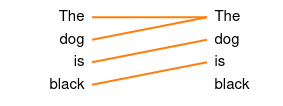
\includegraphics[scale=\myscale,scale=0.5]{figures/attention_l4_h11_01}\qquad 
	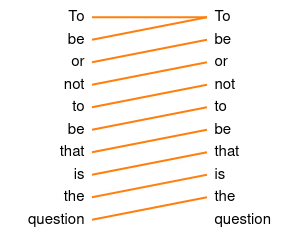
\includegraphics[scale=\myscale,scale=0.5]{figures/attention_l4_h11_02}	
	
	\emph{L'action de la tête d'attention (couche 4, tête 11).}
	
\end{center}

Cette action se visualise immédiatement lorsqu'on relie le mot numéro $i$ (colonne de gauche, la requète) au mot numéro $j$ (colonne de droite, la clé) en traçant un segment plus ou moins visible selon la valeur du coefficient $h_{ij}$ de la matrice d'attention $h$. Ci-dessus (à gauche) on voit clairement que le \mot{␣black} est relié par le mot \mot{␣is} qui le précède. À droite, un autre exemple de cette même tête d'attention avec la phrase \mot{To be or not to be ...}.


Certaines têtes d'attention font correspondre le token en cours avec lui même (couche $0$, tête $3$), d'autres répartissent l'attention entre tous les tokens précédents (couche $0$, tête $9$), ou bien détectent les répétions (couche $0$, tête $5$). 

\begin{center}
	\begin{minipage}{0.3\textwidth}
	\center
	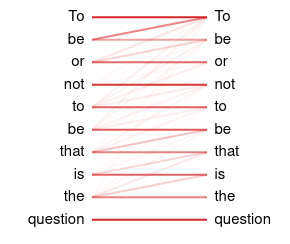
\includegraphics[scale=\myscale,scale=0.5]{figures/attention_l0_h3}
	
	\emph{Couche $0$, tête $3$.}
	\end{minipage}
	\quad
	\begin{minipage}{0.3\textwidth}
	\center
	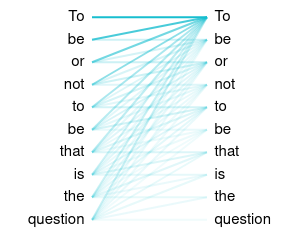
\includegraphics[scale=\myscale,scale=0.5]{figures/attention_l0_h9}
	
	\emph{Couche $0$, tête $9$.}
    \end{minipage}
    \quad
	\begin{minipage}{0.3\textwidth}
	\center
	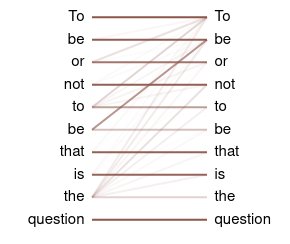
\includegraphics[scale=\myscale,scale=0.5]{figures/attention_l0_h5}
	
	\emph{Couche $0$, tête $5$.}
   \end{minipage}

\end{center}


Les couches le plus hautes correspondent à des concepts plus abstraits (verbes d'actions, repérage spatio-temporel, lien entre un entier $n$ et sont suivant $n+1$, \ldots). Comme d'habitude, il est difficile d'interpréter précisément l'action de chaque objet. 
Certaines têtes font du copier-coller, d'autres jouent le rôle inverse en interdisant les redondances. Si par exemple on souhaite compléter la phrase \og{}\mot{Il visite la France et Paris. Il commence par ...}\fg{} En voyant les termes \mot{visite}, \mot{France}, \mot{Paris} un réseau mal paramétré pourrait par exemple compléter avec \mot{Paris}, ce qui n'est pas complètement illogique mais maladroit. Certaines têtes empêchent de réutiliser un mot déjà rencontré, ainsi le réseau pourrait compléter en \mot{il commence par la tour Eiffel}.



%%%%%%%%%%%%%%%%%%%%%%%%%%%%%%%%%%%%%%%%%%%%%%%%%%%%%%%%%%%%%%%%%%%%%
\section{Fonction d'activation GELU}


%--------------------------------------------------------------------
%\subsection{GELU}

Le choix de la fonction d'activation est primordial pour l'efficacité du calcul par rétropropagation.
Des travaux récents se sont intéressés à des fonctions d'activation plus performantes.
Nous allons étudier la fonction d'activation GELU qui est celle choisie par \emph{GPT2}.

L'idée de départ est que les données étudiées se répartissent souvent en suivant une loi normale (ou loi de Gauss) et pas une loi uniforme. 
On renvoie au chapitre \og{}Probabilités\fg{}.

Rappelons que la \defi{loi de Gauss centrée réduite} est définie par :
$$f(x) = \frac{1}{\sqrt{2\pi}} e^{-\frac12 x^2}.$$
La \defi{fonction de répartition} associée est la primitive de $f$ :
$$\Phi(x) = \frac{1}{\sqrt{2\pi}} \int_{-\infty}^x e^{-\frac12 t^2} \dd t$$
Autrement dit, $\Phi(x)$ est la probabilité de l'événement $f(X \le x)$.


\begin{center}
	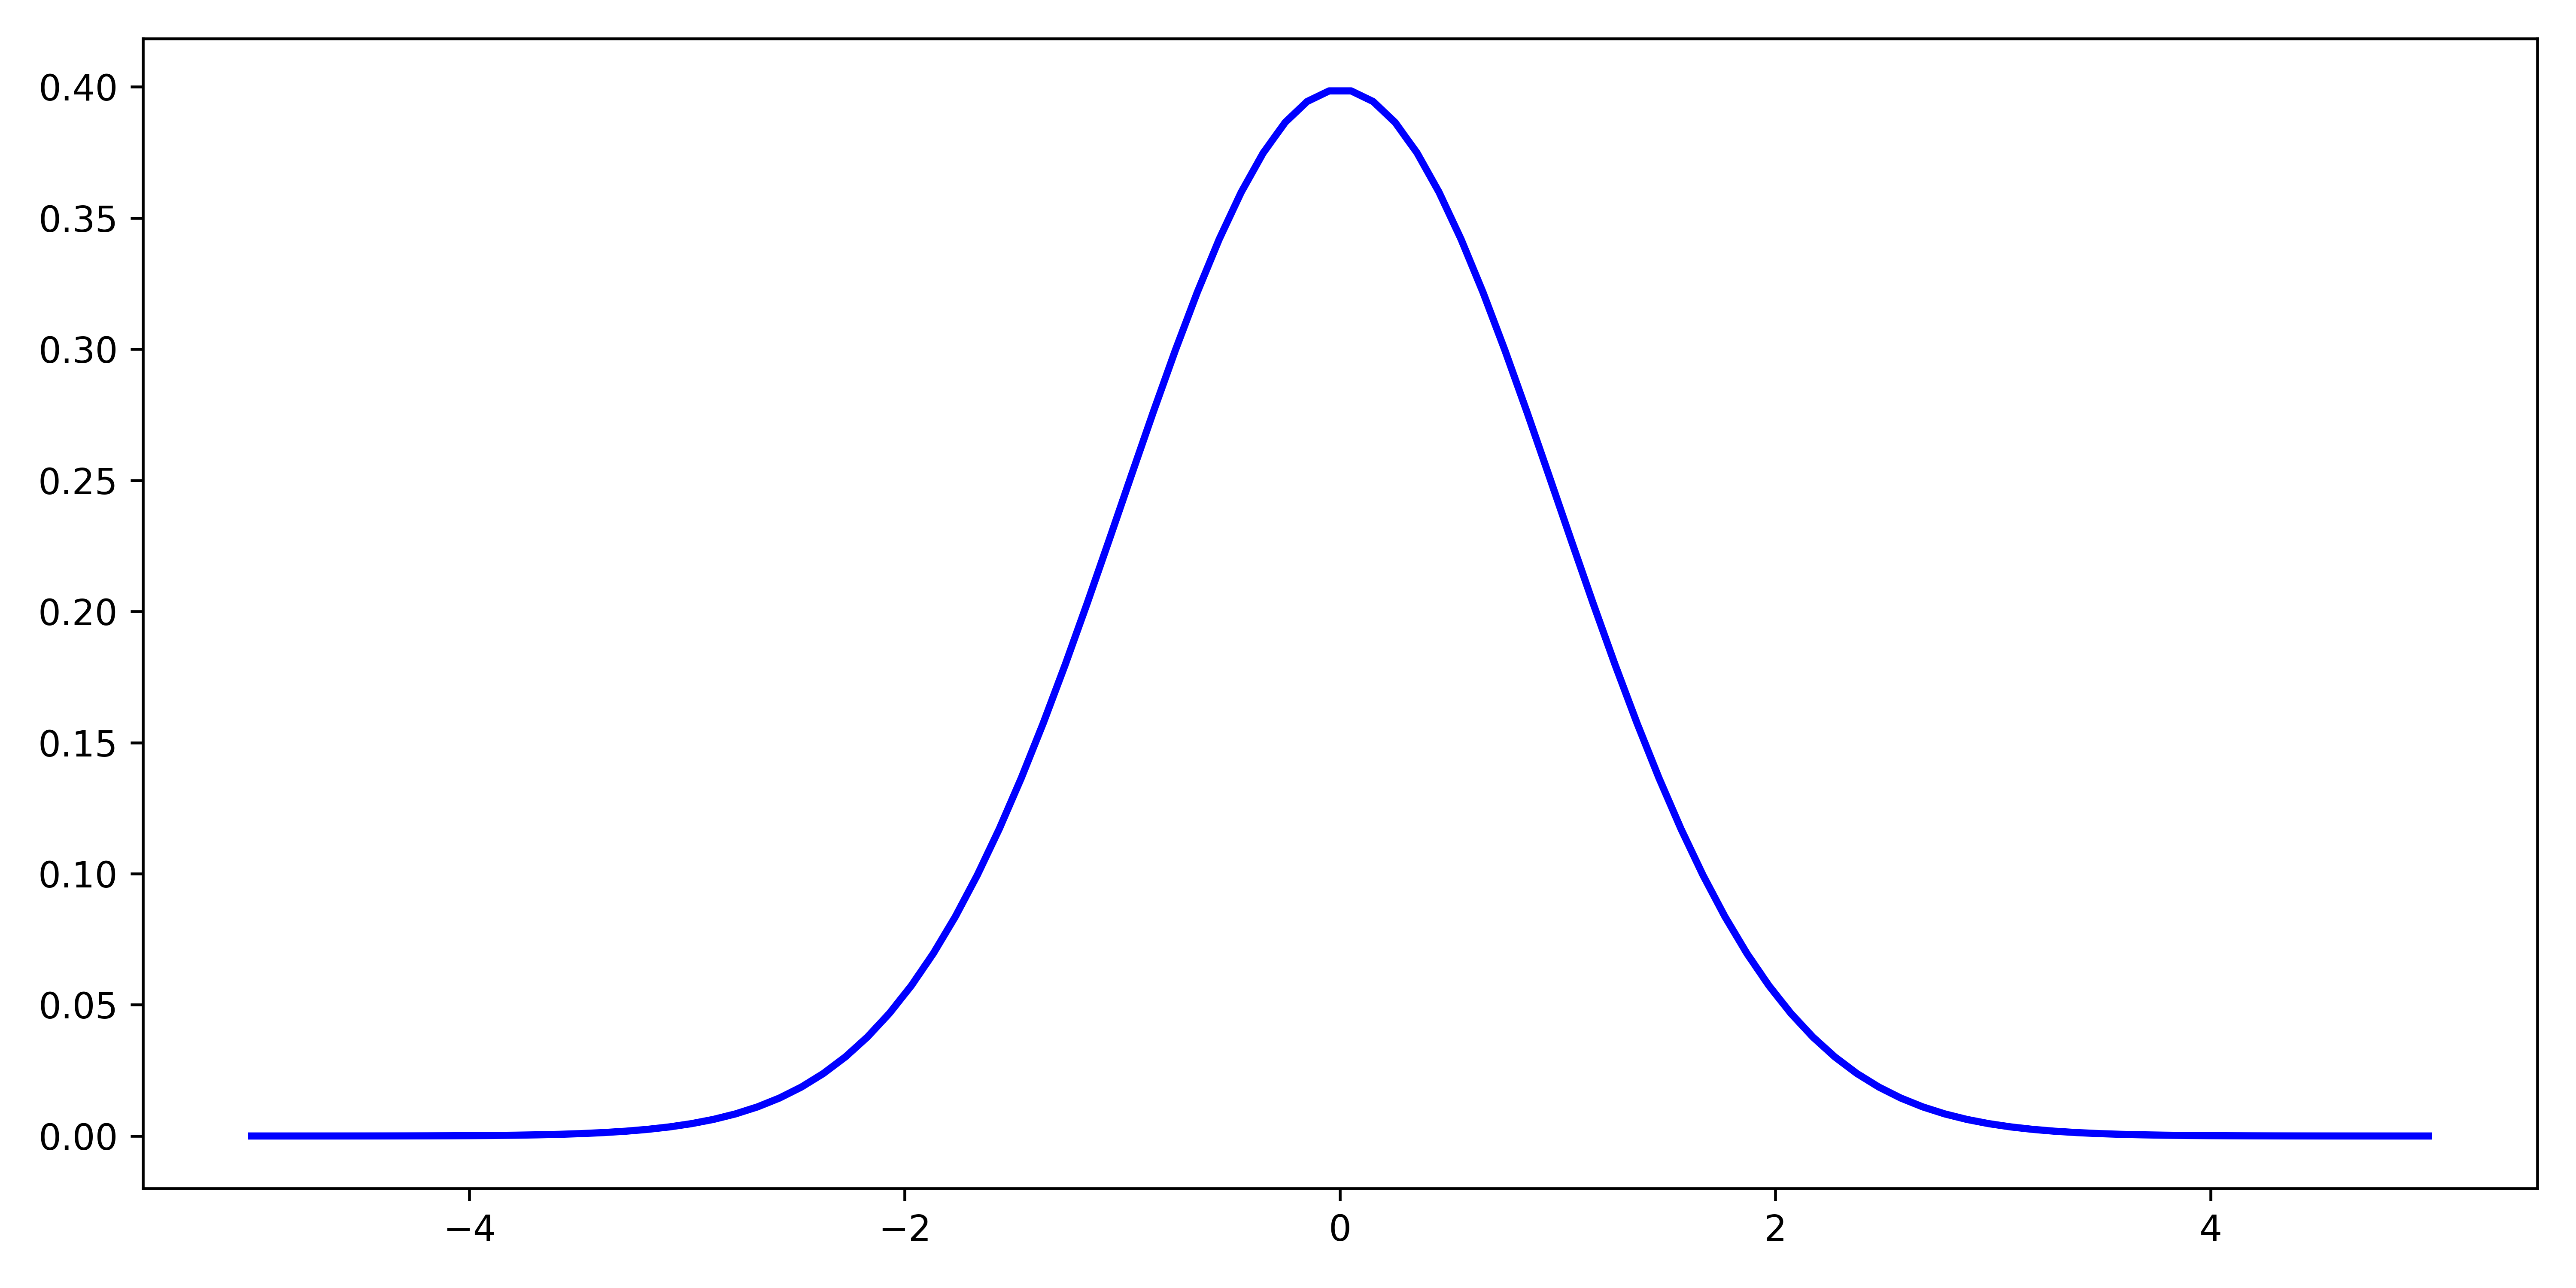
\includegraphics[scale=\myscale,scale=0.3]{figures/gelu01}\quad 
	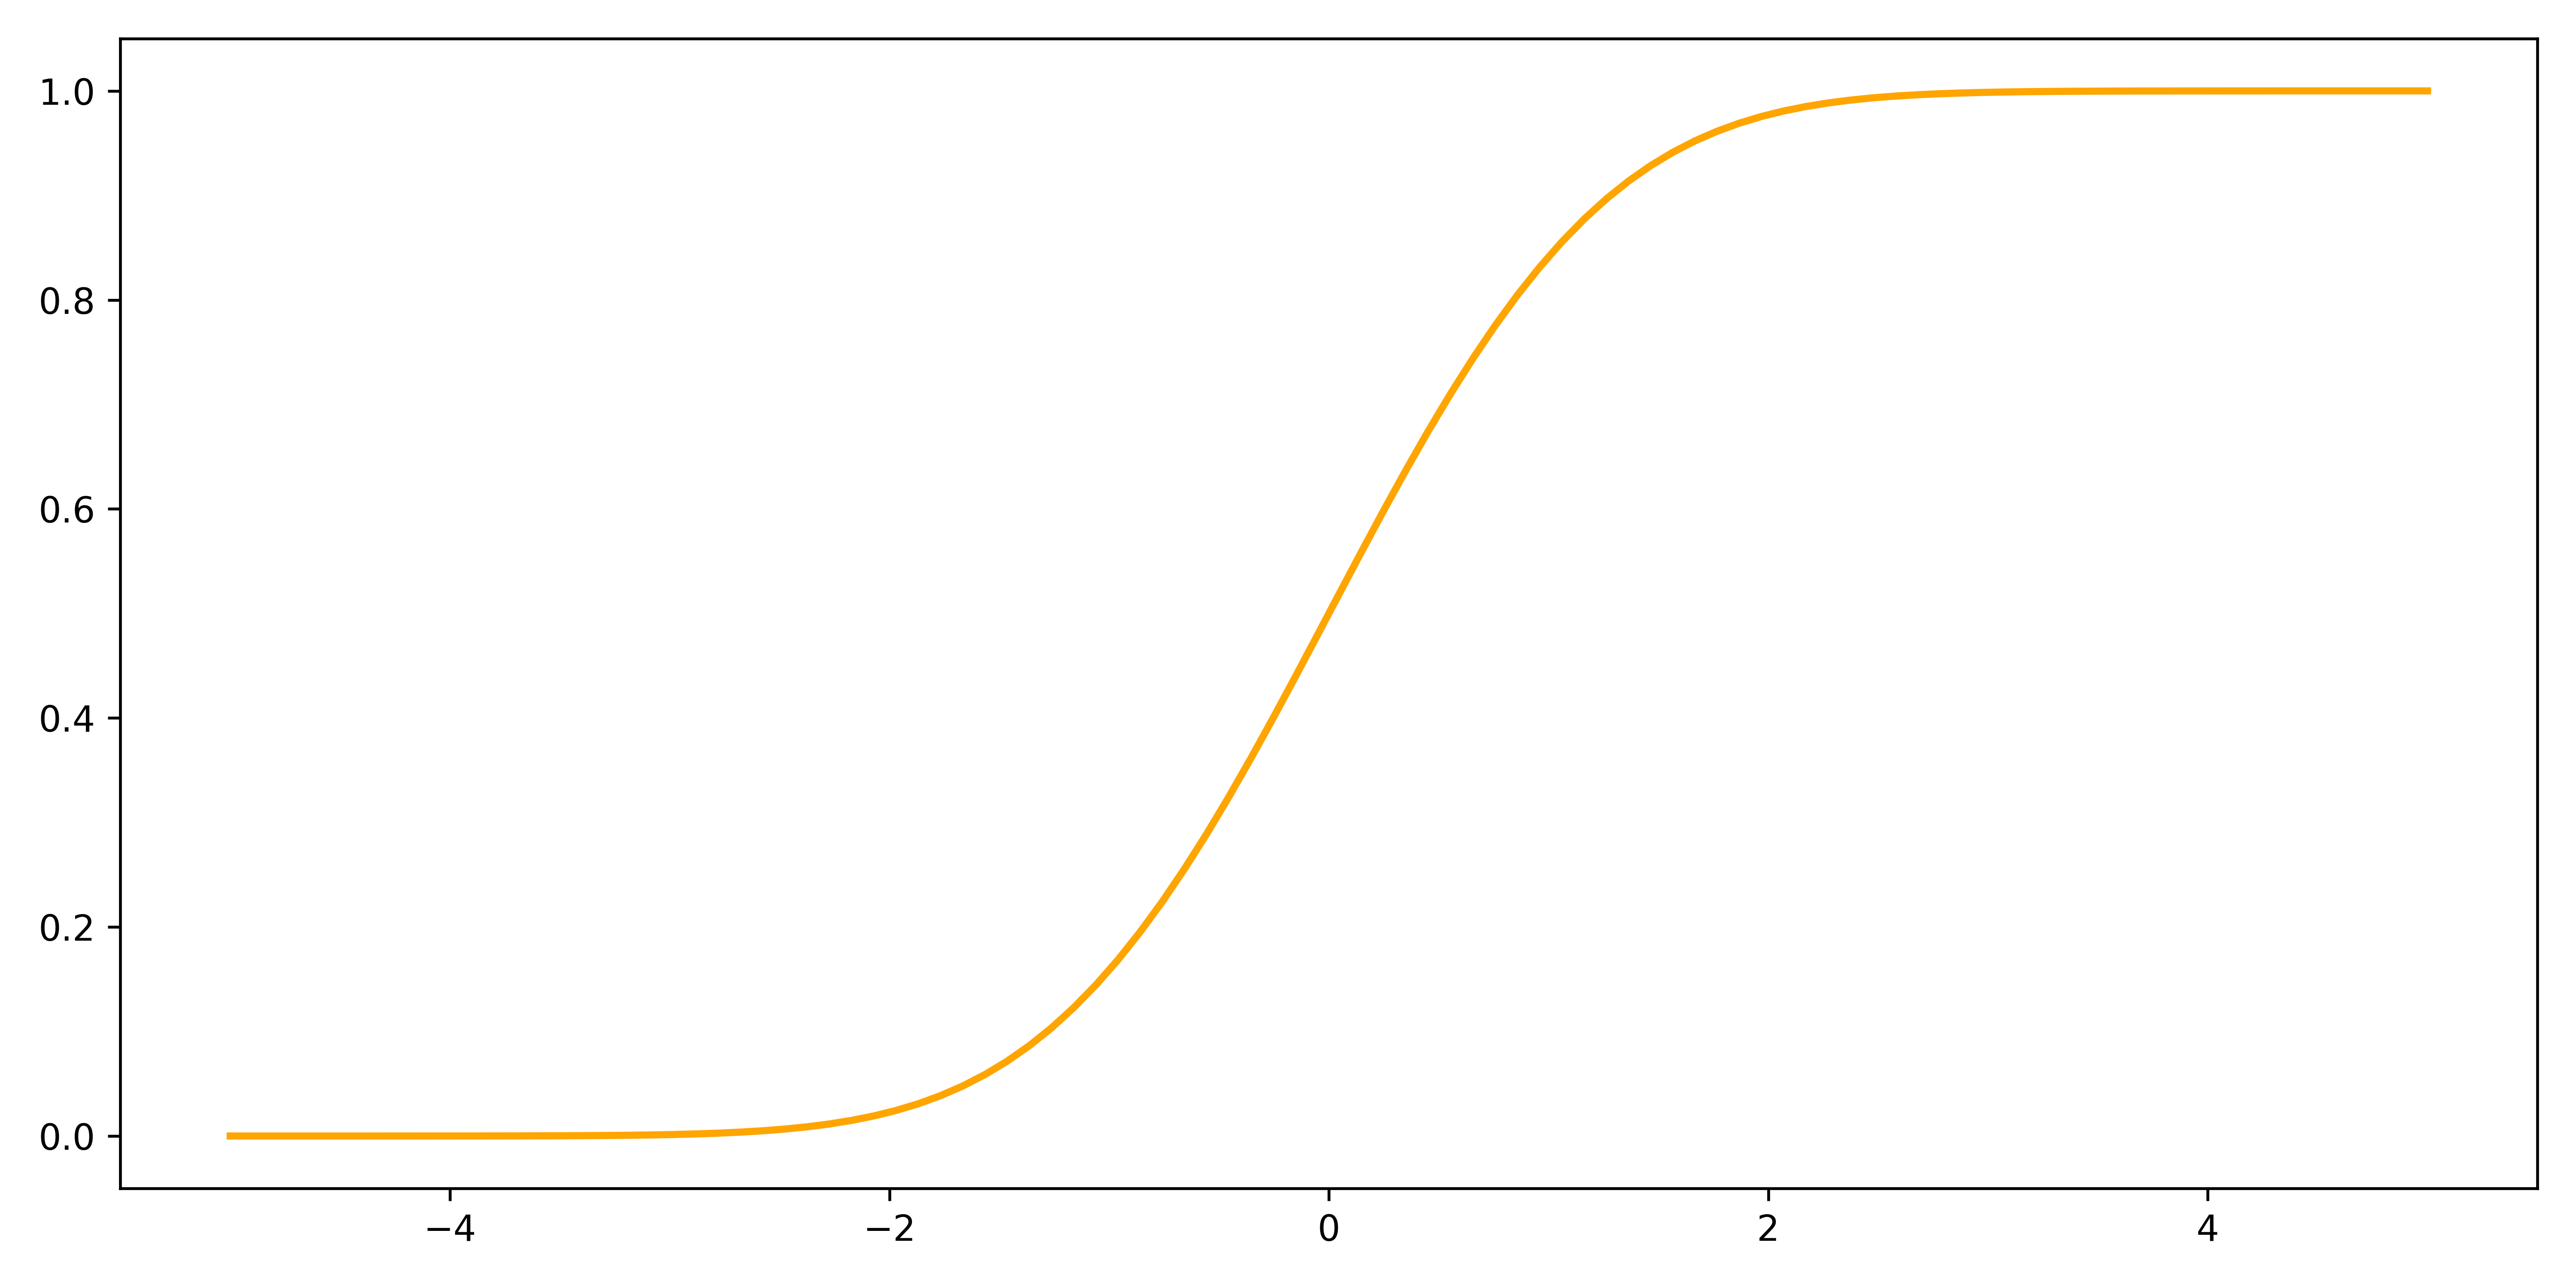
\includegraphics[scale=\myscale,scale=0.3]{figures/gelu02}	
	
	
	\emph{À gauche la fonction $f$ définissant la loi de Gauss, à droite la fonction de répartition $\Phi$.}
	
\end{center}

La fonction \defi{GELU} (pour \emph{Gauss Error Linear Unit}) est défini par 
$$\GELU(x) = x \Phi(x)$$


\begin{center}
	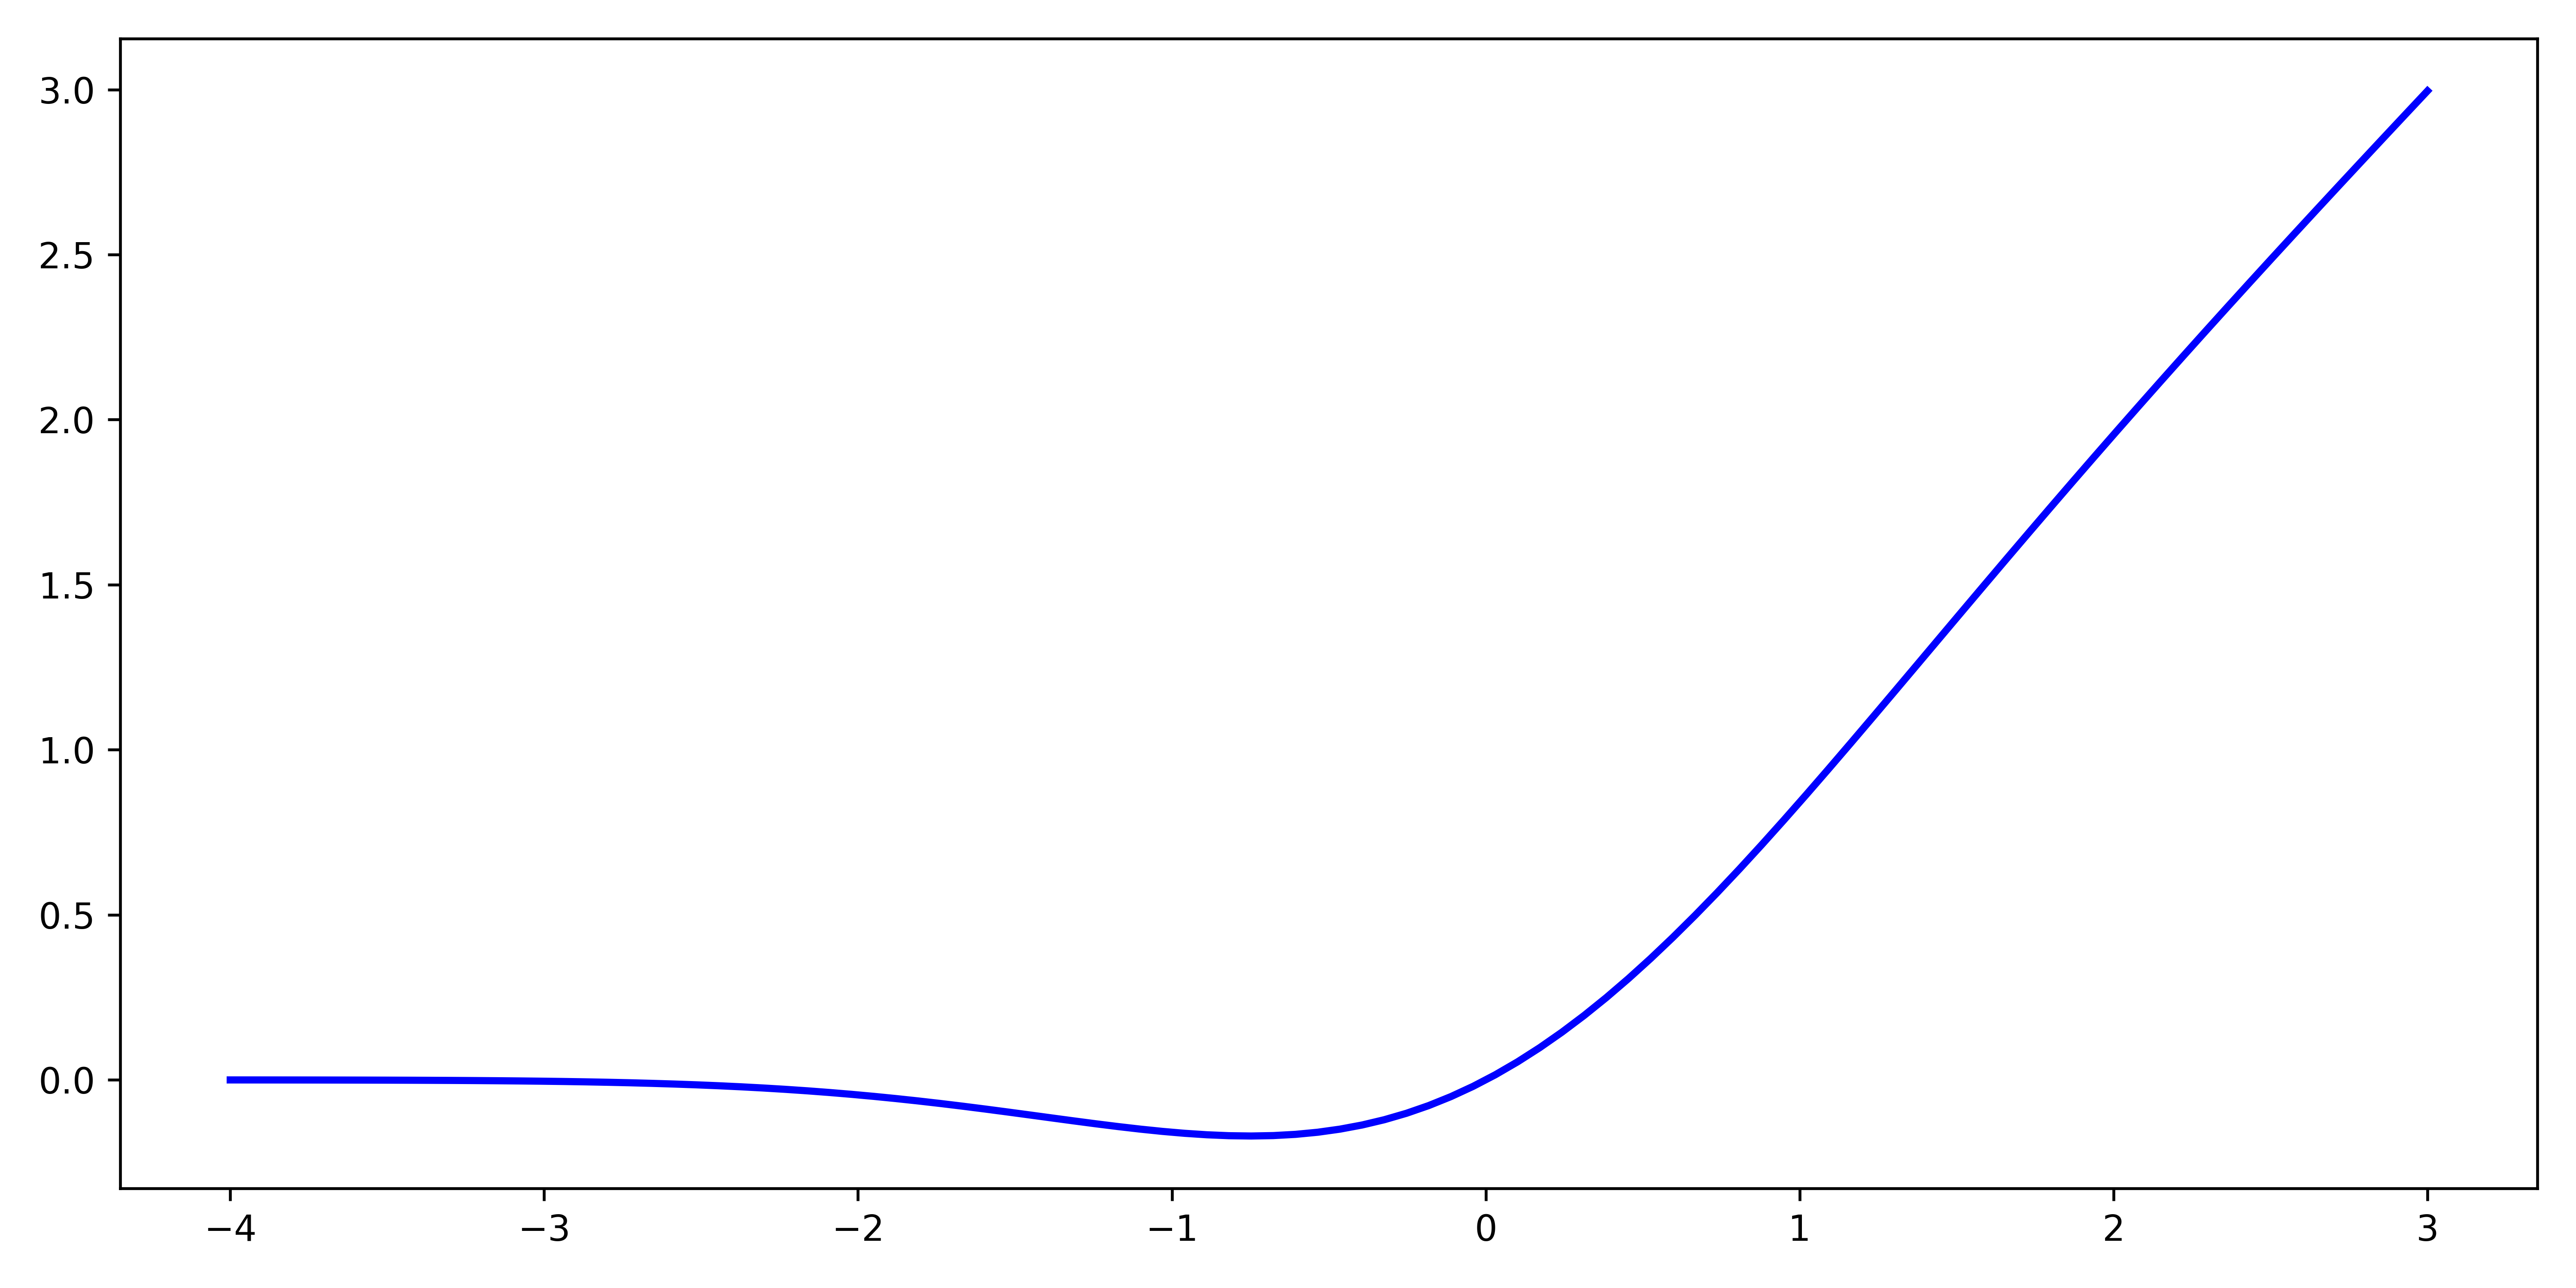
\includegraphics[scale=\myscale,scale=0.3]{figures/gelu03}\quad
	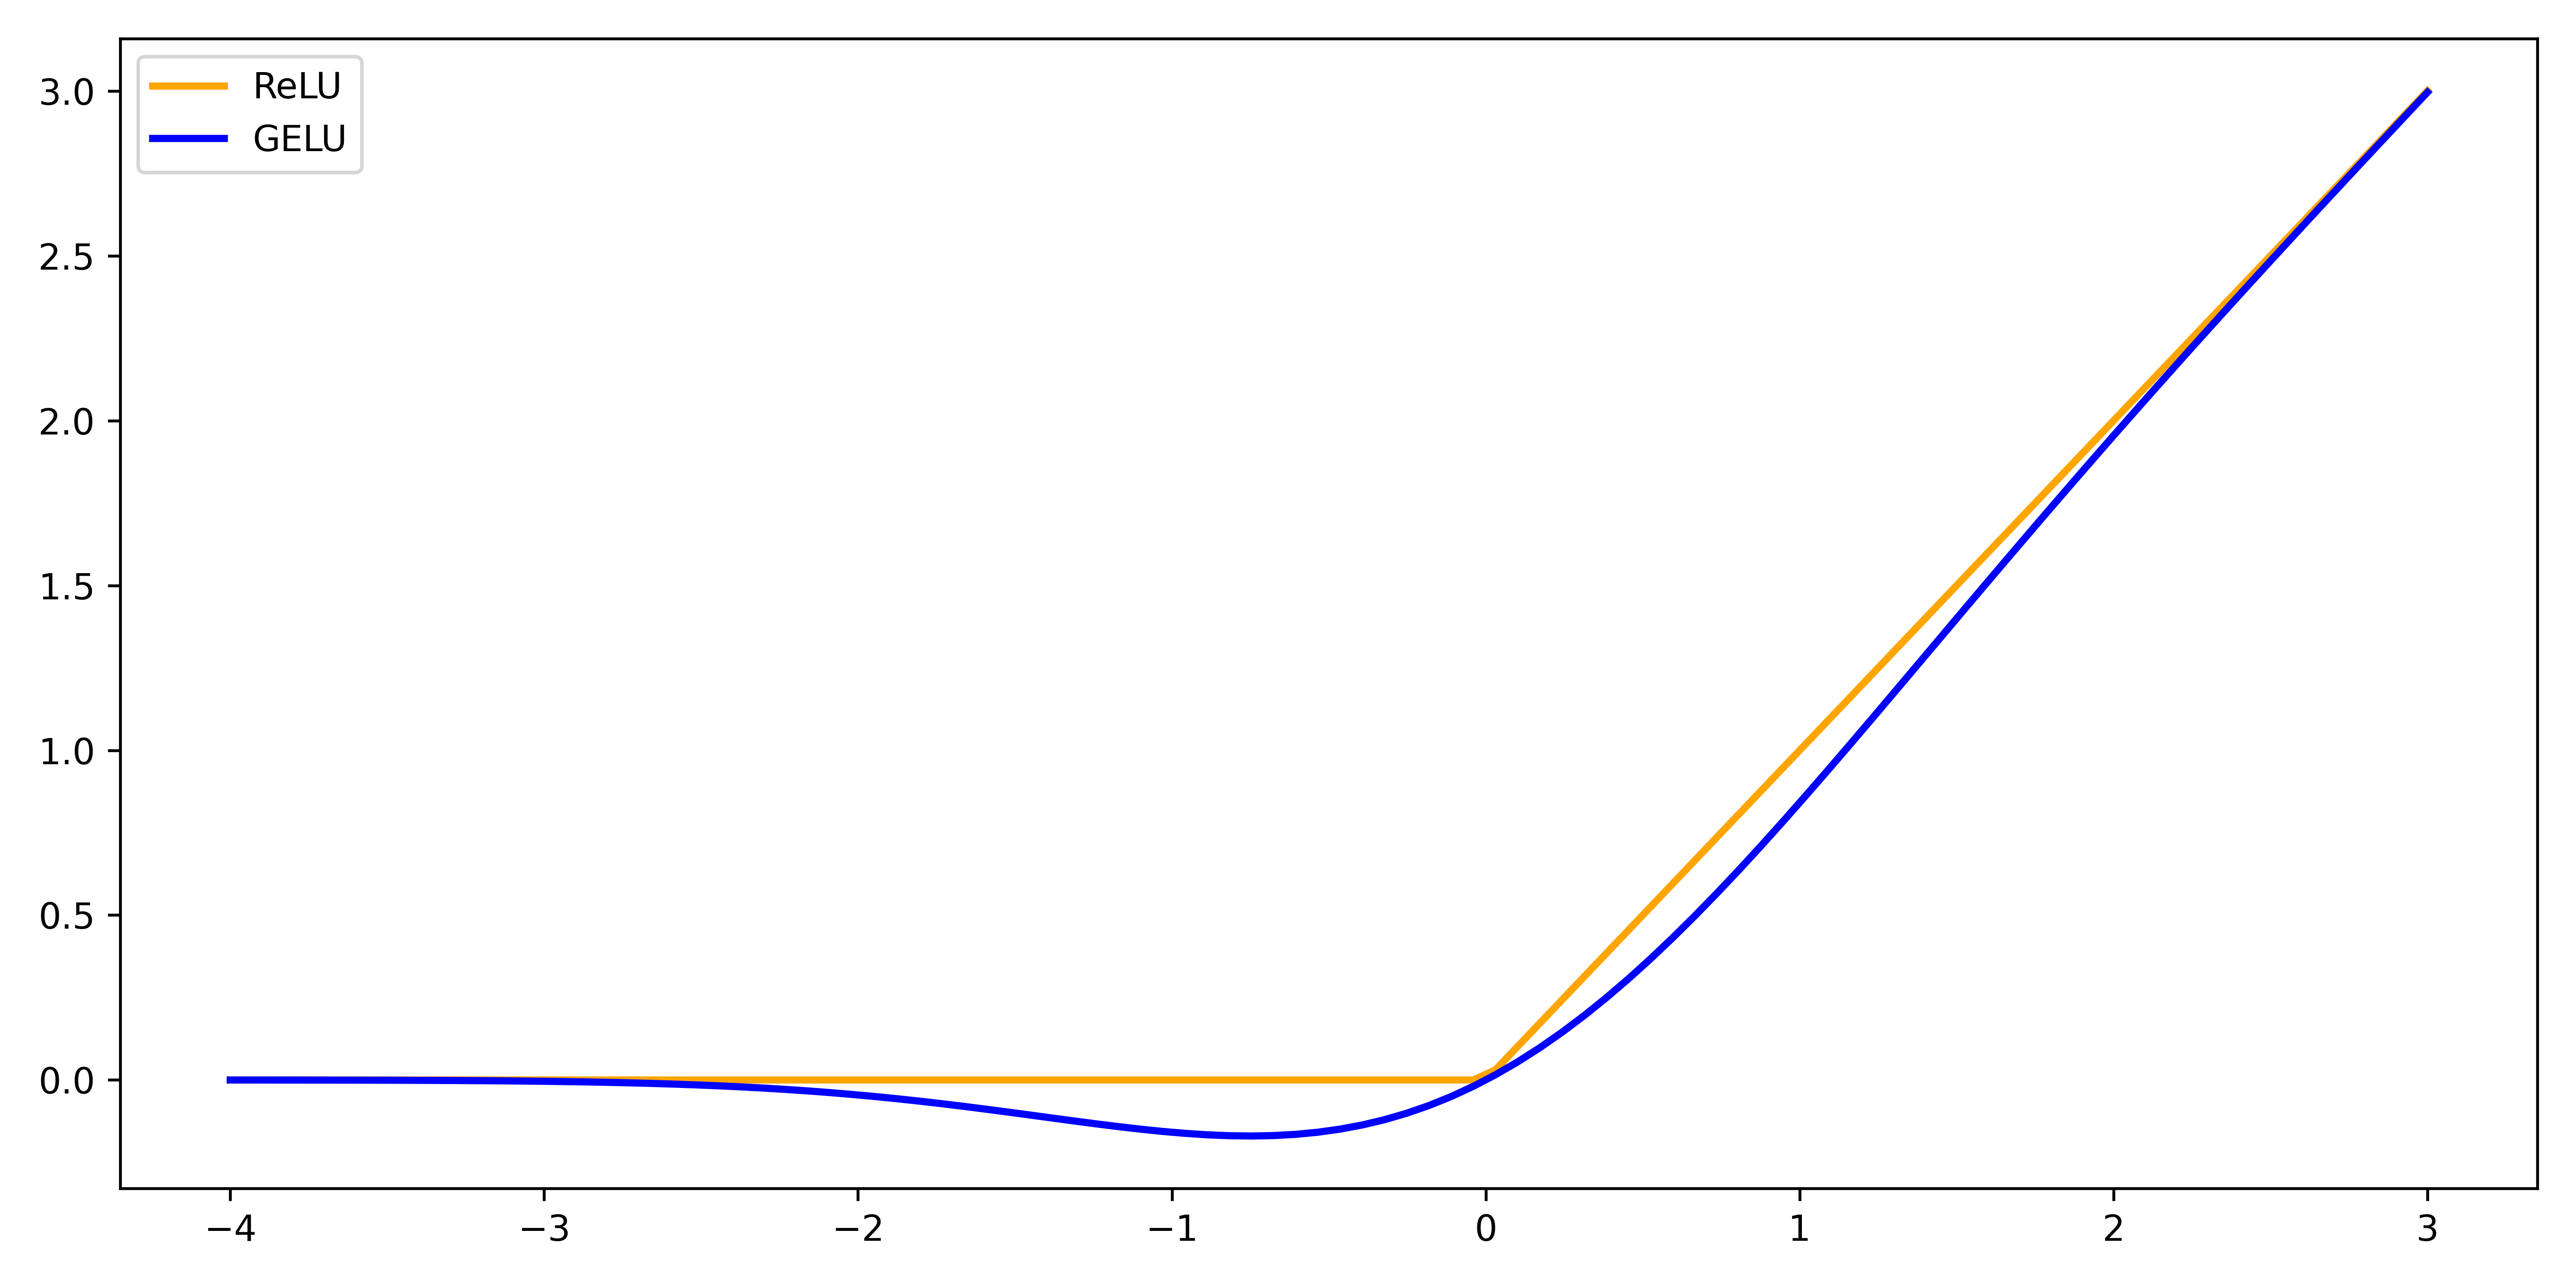
\includegraphics[scale=\myscale,scale=0.3]{figures/gelu04}
	
	\emph{À gauche la fonction GELU, à droite la comparaison avec la fonction ReLU.}	
\end{center}

\textbf{GELU vs ReLU.}

Cette fonction est assez proche de la fonction ReLU.
Cependant ReLU est nulle pour des $x$ négatifs ce qui fait que lors de la rétropropagation beaucoup de poids ne sont pas modifiés à chaque itération et cela représente une perte d'efficacité. 

La fonction GELU a l'avantage d'être dérivable partout (ce qui n'est pas le cas de ReLU en $0$), d'être non nulle (sauf en $0$). Il semble aussi qu'être non-monotone (c'est-à-dire ni croissante, ni décroissante) et avoir des valeurs négatives lui procure un avantage.
Il est difficile de quantifier et de justifier davantage le gain obtenu, cependant expérimentalement GELU est plus performante.

\bigskip

\textbf{Comment calculer GELU ?}

Dans la pratique, après un changement de variable, on préfère exprimer GELU à l'aide d'une intégrale finie:
$$\GELU(x) = \frac{x}{2} \left( 1 + \erf\left(\frac{x}{\sqrt{2}}\right) \right)$$
où $\erf : \Rr \to \Rr$ est la \defi{fonction d'erreur de Gauss} :
$$\erf(x) = \frac{2}{\sqrt \pi} \int_0^x e^{-t^2} \dd t$$

Mais cette fonction $\erf$ ne peut pas s'exprimer de façon exacte à l'aide des fonctions usuelles. Heureusement le calcul approché de cette fonction est déjà implémenté dans tous les langages modernes.

On peut aussi approcher directement la fonction GELU à l'aide des fonctions usuelles :
$$\GELU(x) \simeq \frac{x}{2} \left( 1 + \tanh\left( \sqrt{\tfrac{2}{\pi}} + 0.44715 x^3 \right)\right)$$
où on rappelle que la \defi{tangente hyperbolique} est définie par $\tanh(x) = \frac{e^x - e^{-x}}{e^x + e^{-x}}$.

Une autre approximation utilise la fonction sigmoïde $\sigma(x) = \frac{1}{1+e^{-x}}$ avec :
$$\GELU(x) \simeq x\sigma(1.702 x)$$


\begin{center}
	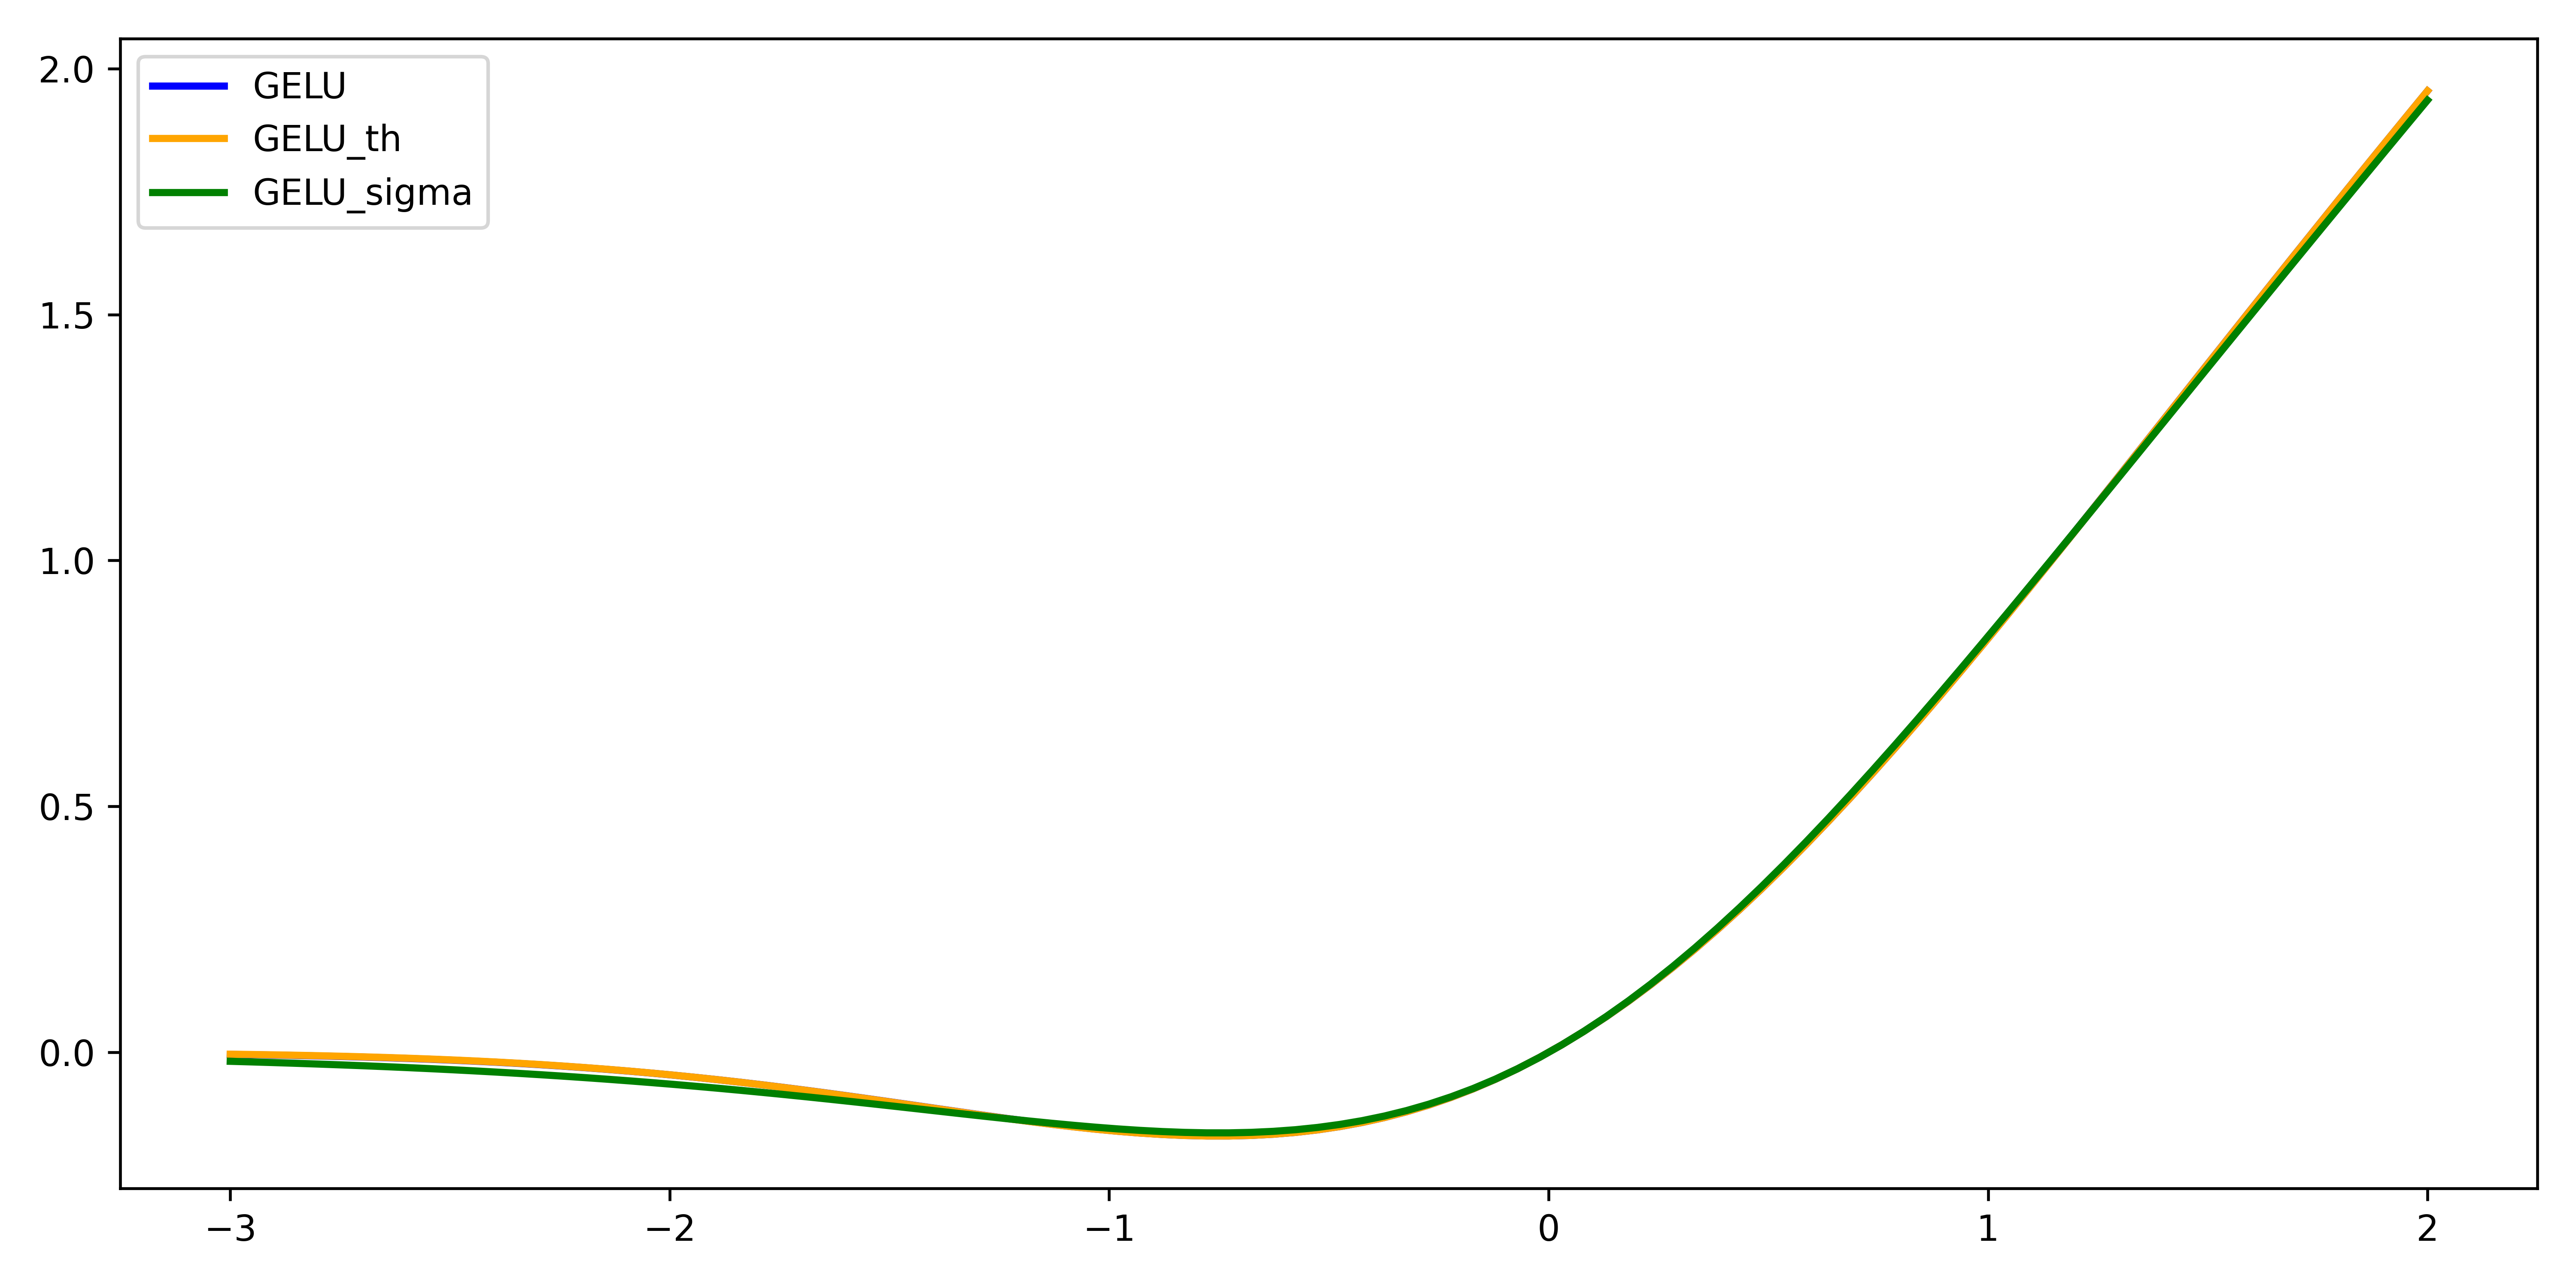
\includegraphics[scale=\myscale,scale=0.3]{figures/gelu05}\quad
	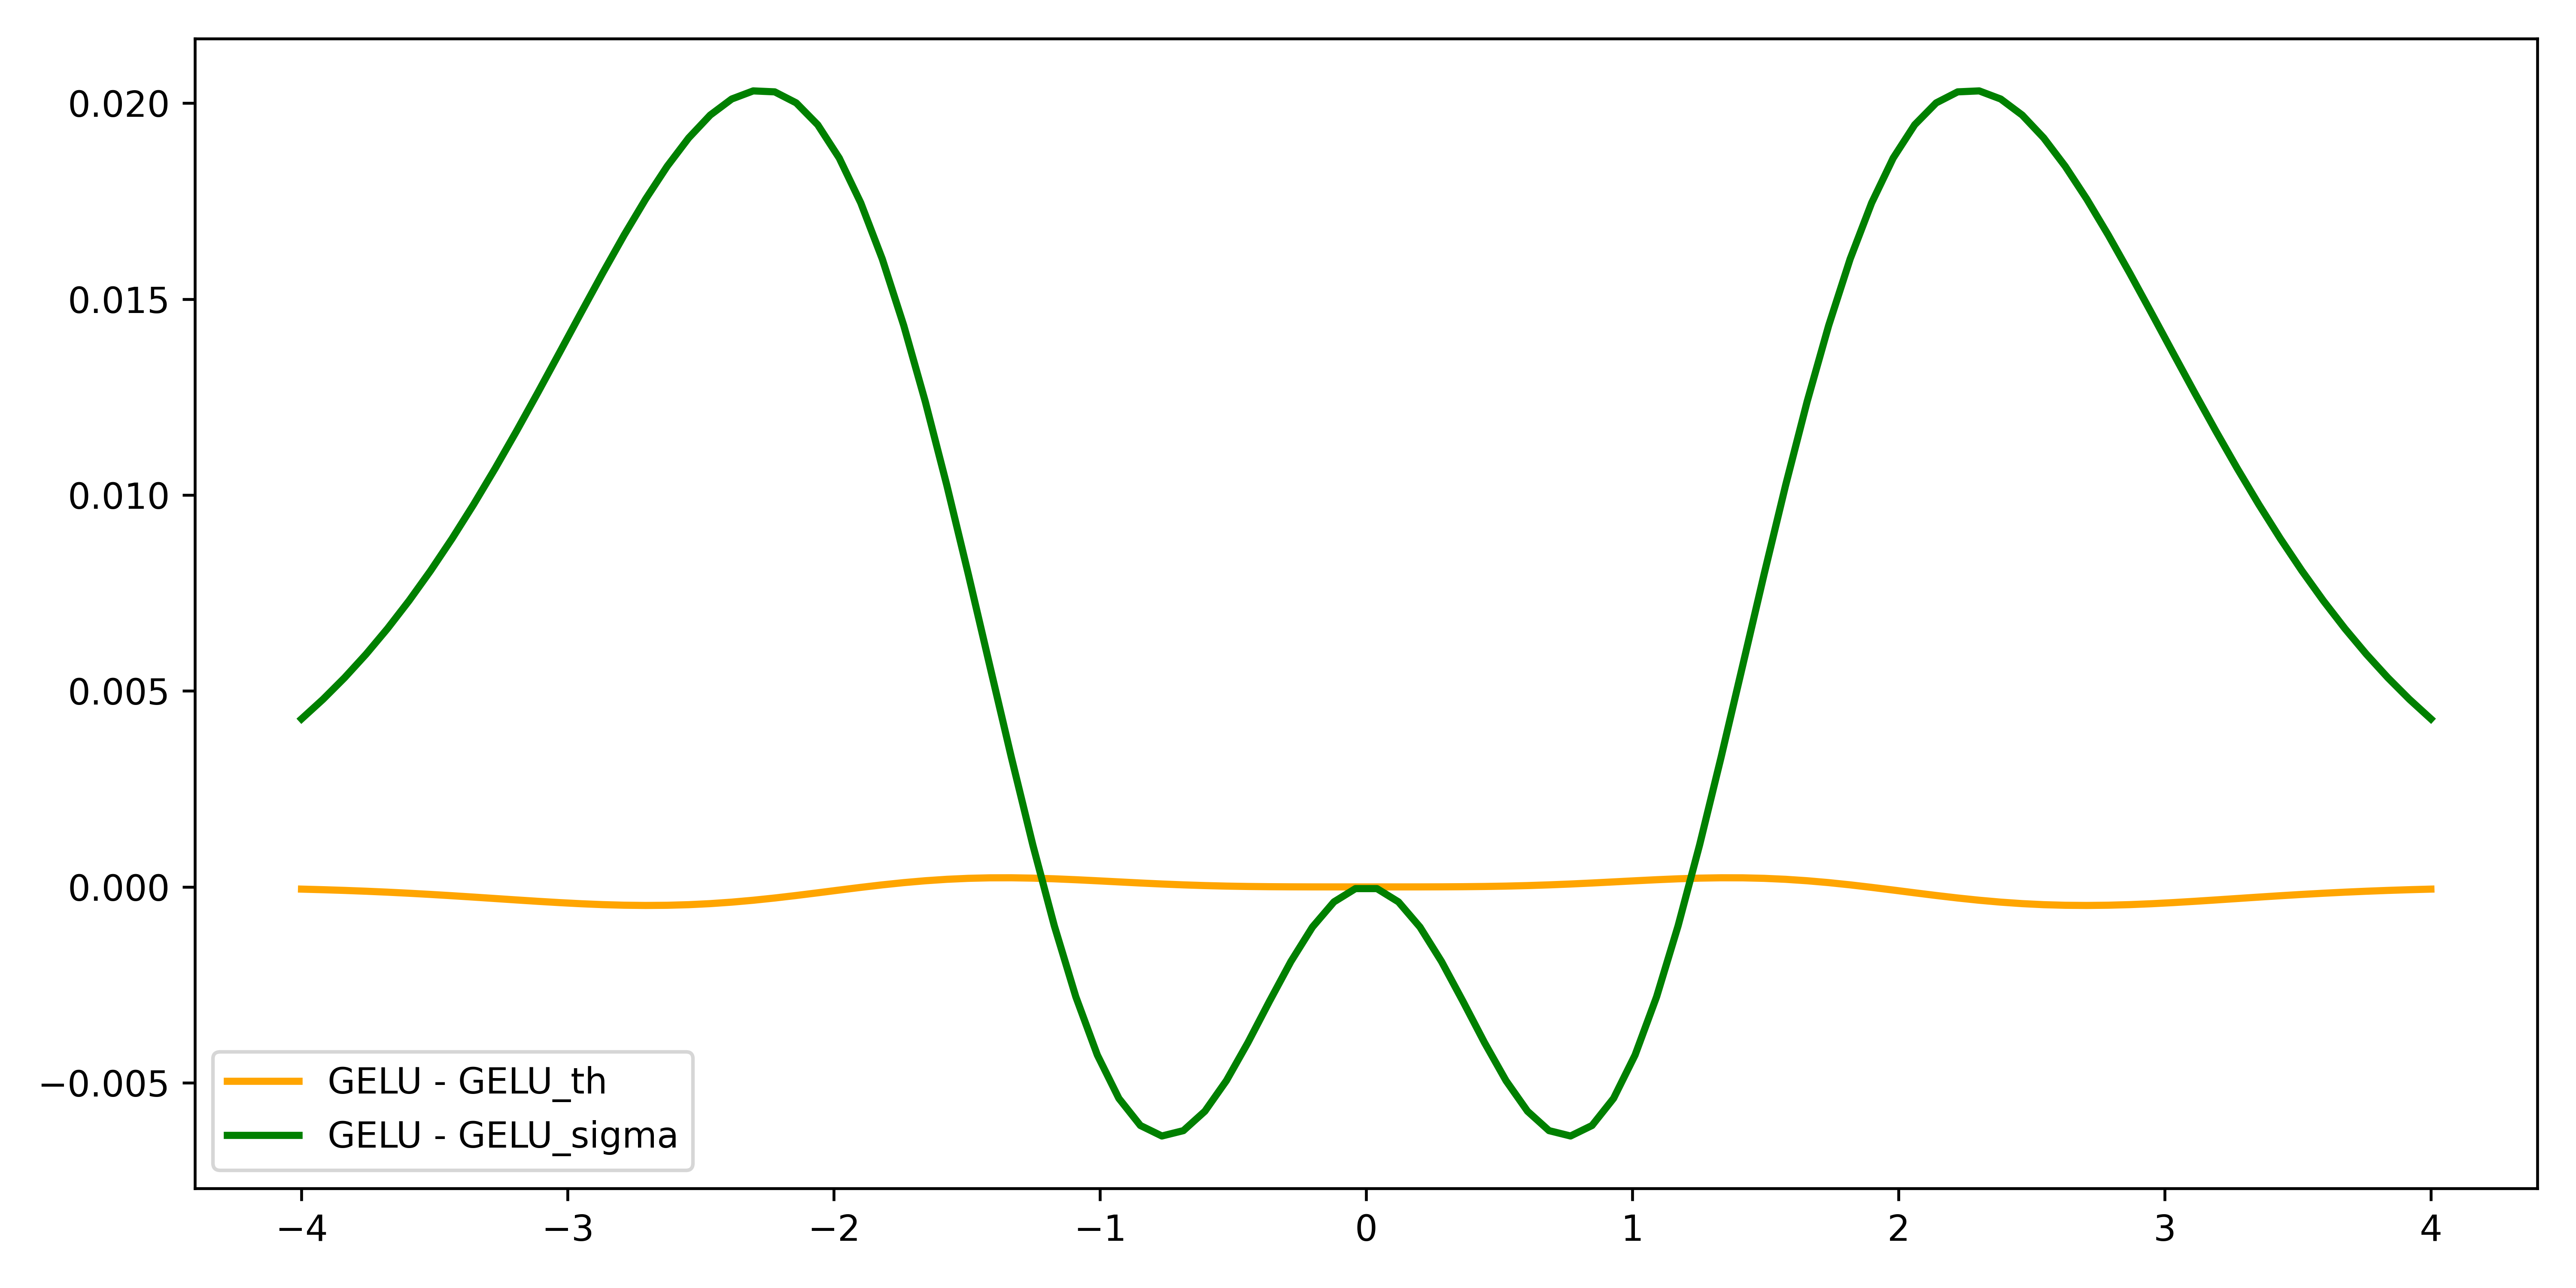
\includegraphics[scale=\myscale,scale=0.3]{figures/gelu06}	
	
	\emph{À gauche, la fonction GELU et ses deux approximations sont indiscernables, à droite l'erreur commise par chacune des ces deux approximations.}
\end{center}

\vfill

Références : l'article fondateur est 
\href{https://arxiv.org/pdf/1706.03762.pdf}{\emph{Attention is all you need}}, des explications mathématiques se trouvent dans
\href{https://transformer-circuits.pub/2021/framework/index.html}{\emph{A mathematical framework for transformer circuits}}.

\bigskip


\end{document}
